% ============================================================
% Psych-Bench: A Comprehensive Cognitive Battery for Evaluating
%   Holographic Liquid Brain Architectures
%
% Target venue: Behavior Research Methods (BRM)
% ============================================================
\documentclass[11pt,letterpaper]{article}

% --- Page layout ---
\usepackage[margin=1in]{geometry}
\usepackage{setspace}
\doublespacing
\usepackage[right]{lineno}
\linenumbers

% --- Typography ---
\usepackage{microtype}
\usepackage[T1]{fontenc}
\usepackage[utf8]{inputenc}

% --- Math ---
\usepackage{amsfonts,amsmath,amssymb}

% --- Tables ---
\usepackage{booktabs}
\usepackage{multirow}
\usepackage{array}
\usepackage{longtable}
\usepackage{tabularx}

% --- Figures ---
\usepackage{graphicx}
\usepackage{float}
\usepackage{tikz}
\usepackage{pgfplots}
\usepackage{pgfplotstable}
\pgfplotsset{compat=1.18}
\usetikzlibrary{arrows.meta,positioning,shapes.geometric,decorations.pathreplacing,calc,patterns}

% --- Color ---
\usepackage[dvipsnames]{xcolor}
\definecolor{hlbblue}{HTML}{2E86C1}
\definecolor{hlbgreen}{HTML}{27AE60}
\definecolor{hlbred}{HTML}{E74C3C}
\definecolor{hlbyellow}{HTML}{F39C12}
\definecolor{hlbpurple}{HTML}{8E44AD}
\definecolor{hlbgray}{HTML}{7F8C8D}
\definecolor{humanband}{HTML}{D5E8D4}

% --- References ---
\usepackage[authoryear,round]{natbib}

% --- Hyperlinks ---
\usepackage[colorlinks=true,linkcolor=hlbblue,citecolor=hlbblue,urlcolor=hlbblue]{hyperref}

% --- Lists ---
\usepackage{enumitem}

% --- Subcaptions ---
\usepackage{subcaption}

% --- Code listings ---
\usepackage{listings}
\lstdefinelanguage{Rust}{
    morekeywords={use,let,fn,for,in,if,else,pub,struct,impl,mod,crate,self,mut,ref,match,return,as,where,type,trait,enum,const,static,move,async,await,dyn},
    sensitive=true,
    morecomment=[l]{//},
    morecomment=[s]{/*}{*/},
    morestring=[b]",
}
\lstset{
    language=Rust,
    basicstyle=\ttfamily\scriptsize,
    keywordstyle=\bfseries\color{hlbblue},
    commentstyle=\itshape\color{hlbgray},
    stringstyle=\color{hlbgreen},
    breaklines=true,
    frame=single,
    framerule=0.4pt,
    xleftmargin=1em,
    framexleftmargin=0.5em,
    numbers=none,
    aboveskip=0.5\baselineskip,
    belowskip=0.5\baselineskip,
}

% --- Custom commands ---
\newcommand{\hv}{\mathbf{h}}
\newcommand{\bind}{\otimes}
\newcommand{\bundle}{\oplus}
\newcommand{\similar}{\delta}
\newcommand{\dimHDC}{16{,}384}
\newcommand{\symthaea}{\textsc{Symthaea}}
\newcommand{\psychbench}{\textsc{Psych-Bench}}
\newcommand{\hlb}{\textsc{HLB}}

% --- Document ---
\begin{document}

\title{\psychbench{}: A Comprehensive Cognitive Battery for Evaluating\\
Holographic Liquid Brain Architectures}

\author{Tristan Stoltz\\
Luminous Dynamics\\
\texttt{tristan.stoltz@evolvingresonantcocreationism.com}}

\date{}
\maketitle

% ============================================================
% ABSTRACT
% ============================================================
\begin{abstract}
\noindent
We present \psychbench{}, a psychological benchmark suite comprising 143 benchmarks across 27 cognitive domains for evaluating Holographic Liquid Brain (\hlb{}) architectures---systems combining Hyperdimensional Computing, Liquid Time-Constant networks, Integrated Information Theory, and Active Inference. Existing AI evaluation frameworks lack psychometric infrastructure (HELM), cover narrow domains (ARC), omit normative human comparison (BIG-Bench), or ignore neuromodulatory effects (CogBench). \psychbench{} addresses all four gaps with: (1)~implementations of established paradigms (Stroop, WCST, N-back, and 140 others) with psychometric assessment infrastructure including ICC reliability, speed-accuracy tradeoff curves, and adaptive staircases; (2)~normative anchoring against 99 published human baselines enabling z-score and clinical-band interpretation; (3)~a 17-benchmark neuromodulator evaluation framework testing dose-response curves, tolerance/withdrawal dynamics, behavioral knockouts, and multi-transmitter synergy; and (4)~a 14-indicator consciousness evaluation derived from six theories. All stimuli share a unified holographic encoding via five HDC adapter types, enabling cross-modal comparison. Demonstration on the \symthaea{} \hlb{} reveals a grand mean z-score of $+1.32$ across 27 cognitive domains (27/27 above human mean, 0 below), with cross-seed stability SD~$= 0.065$ (5 seeds). Particular strengths emerge in Motor ($z = +2.32$), InstitutionalReasoning ($z = +2.25$), SustainedAttention ($z = +2.19$), Speech ($z = +2.13$), Clinical ($z = +2.00$), and Security ($z = +2.00$). Psychometric analysis reveals a gradient of reliability from Excellent to Poor (5 Excellent, 4 Good, 2 Moderate, 9 Poor across 20 evaluated benchmarks), selective sensitivity to working-memory and encoding-noise ablation, and accuracy-pressure tradeoffs in 4 of 8 tested benchmarks. Implemented in ${\sim}20{,}000$ lines of Rust with 1,283 unit tests, \psychbench{} is open-source and fully deterministic.
\end{abstract}

\paragraph{Keywords:} cognitive benchmark, holographic computing, liquid neural networks, neuromodulation, psychometrics, consciousness evaluation, hyperdimensional computing

% ============================================================
% 1. INTRODUCTION
% ============================================================
\section{Introduction}
\label{sec:introduction}

A new class of cognitive architecture has emerged at the intersection of hyperdimensional computing, dynamical systems neuroscience, and consciousness science. These \emph{Holographic Liquid Brain} (\hlb{}) architectures encode information as high-dimensional distributed representations---the ``holographic'' component, drawing on Plate's holographic reduced representations~\citep{plate1995holographic} and Kanerva's hyperdimensional computing framework~\citep{kanerva2009hyperdimensional}---while processing temporal dynamics through liquid-state computation, specifically Liquid Time-Constant (LTC) networks~\citep{hasani2021liquid} and their closed-form continuous-time variant (CfC)~\citep{hasani2022closed}. The ``liquid'' component provides biologically plausible temporal processing with continuous-time dynamics and adaptive time constants, while integration with Integrated Information Theory (IIT)~\citep{tononi2004information,oizumi2014phenomenology} and Active Inference under the Free Energy Principle~\citep{friston2010free,friston2017active} creates architectures with rich internal dynamics that demand correspondingly rich evaluation.

The fundamental challenge is methodological: how should we evaluate cognitive architectures that aspire to neuroscience-grade fidelity? Standard AI benchmarks fall short in four critical ways.

\paragraph{Lack of psychometric rigor.} The Holistic Evaluation of Language Models (HELM)~\citep{liang2023holistic} evaluates across many tasks but treats each as an isolated accuracy measure without psychometric validation---no test-retest reliability, no construct validity analysis, no speed-accuracy decomposition. A benchmark that fluctuates wildly across runs tells us nothing stable about the architecture it evaluates.

\paragraph{Narrow domain coverage.} The Abstraction and Reasoning Corpus (ARC)~\citep{chollet2019measure} provides an excellent measure of fluid intelligence but covers a single cognitive domain. Human cognition is characterized by the interplay between executive function, working memory, social cognition, motor learning, and dozens of other capacities. Single-domain benchmarks cannot capture the profile that emerges from an integrated architecture.

\paragraph{Absence of normative comparison.} BIG-Bench~\citep{srivastava2023beyond} offers hundreds of tasks but provides no systematic comparison to human performance distributions. Without normative anchoring---z-scores against published baselines with known means and standard deviations---we cannot interpret whether an architecture's performance on a given task is exceptional, average, or impaired relative to the human population it models.

\paragraph{The neuromodulator gap.} Perhaps most critically, no existing benchmark suite tests the effects of pharmacological manipulations on cognitive performance. CogBench~\citep{codaforno2024cogbench} applies eight cognitive psychology paradigms to large language models, representing the closest existing work, but its eight tasks and prompt-based interface cannot probe neuromodulatory dynamics. For \hlb{} architectures with explicit dopaminergic, noradrenergic, serotonergic, and cholinergic subsystems, evaluating how these transmitters modulate behavior is essential---analogous to how pharmacological challenge studies validate computational models of the basal ganglia~\citep{doya2002metalearning} or prefrontal cortex~\citep{arnsten2011catecholamine}.

\psychbench{} addresses all four gaps simultaneously. We present a comprehensive cognitive battery of 143 benchmarks spanning 27 domains, designed specifically for evaluating \hlb{} and related neuroscience-inspired architectures. The suite is organized around five design principles: psychometric fidelity to source paradigms, unified holographic stimulus encoding, normative anchoring against published baselines, systematic ablation transparency, and self-contained reporting.

Our contributions are:
\begin{enumerate}[nosep]
    \item A 143-benchmark cognitive battery covering 27 cognitive domains including executive function, working memory, attention, social cognition, motor learning, language, metacognition, reasoning, clinical psychology, institutional reasoning, mathematics, causal reasoning, spatial cognition, and specialized sub-batteries for affect, creativity, inhibition, consciousness, speech, substrate independence, security (FHE), and game-theoretic social cognition.
    \item A 17-benchmark neuromodulator evaluation framework---the first to test pharmacological manipulations (dose-response curves, injection challenges, tolerance/withdrawal, antagonist profiles, multi-transmitter synergy) in an AI benchmark context.
    \item A psychometric infrastructure providing ICC(3,1) reliability, ex-Gaussian RT decomposition~\citep{heathcote1996fitting}, Wickelgren SAT curves~\citep{wickelgren1977speed}, adaptive staircases~\citep{levitt1971transformed}, and normative z-score comparison with clinical interpretation bands~\citep{cicchetti1994guidelines}.
    \item A 14-indicator consciousness evaluation derived from Butlin et al.'s~\citep{butlin2023consciousness} six-theory framework, with ablation matrices linking architectural features to indicator presence.
\end{enumerate}

% ============================================================
% 2. DESIGN PRINCIPLES
% ============================================================
\section{Design Principles}
\label{sec:principles}

\psychbench{} is organized around five principles that distinguish it from existing AI evaluation suites.

\paragraph{Psychometric fidelity.} Each benchmark implements the exact experimental paradigm described in its source publication. The Stroop task~\citep{stroop1935interference} presents congruent and incongruent color-word stimuli following MacLeod's~\citep{macleod1991half} standardized procedure. The Wisconsin Card Sorting Test~\citep{berg1948simple} implements 6-category set-shifting with perseverative error tracking. The Iowa Gambling Task~\citep{bechara1994insensitivity} uses the original reward/punishment schedule across 100 trials with four decks. This is not approximation---each benchmark carries a citation to its source paradigm, and the implementation can be audited against the original procedure.

\paragraph{Holographic stimulus encoding.} All stimuli pass through a unified Hyperdimensional Computing (HDC) encoding pipeline before reaching the cognitive architecture. Five adapter types---\texttt{SequenceAdapter}, \texttt{SemanticAdapter}, \texttt{SpatialAdapter}, \texttt{ScenarioAdapter}, and \texttt{RewardAdapter}---convert raw stimuli (token sequences, spatial coordinates, reward outcomes, scenarios) into continuous hypervectors in $\mathbb{R}^D$ using binding ($\bind$) and bundling ($\bundle$) operations~\citep{kleyko2023survey}. This unified representation is the ``holographic'' in \hlb{}: all modalities share a common geometric space where similarity is cosine distance, enabling cross-modal retrieval and comparison. The default dimension $D = 512$ balances representational capacity against computational cost for benchmark-scale evaluation.

\paragraph{Normative anchoring.} Every benchmark has at least one associated human baseline from the published literature, stored as a mean $\pm$ SD pair with citation. The \texttt{BaselineCollection} contains 140+ such entries spanning all 27 domains. Agent performance is converted to z-scores ($z = (x_{\text{agent}} - \mu_{\text{human}}) / \sigma_{\text{human}}$, negated for error metrics where lower is better) and mapped to percentiles via the normal cumulative distribution function. Clinical interpretation bands follow Cicchetti's~\citep{cicchetti1994guidelines} guidelines: Superior ($z > 2.0$), Above Average ($1.0 < z \leq 2.0$), Average ($-1.0 \leq z \leq 1.0$), Below Average ($-2.0 \leq z < -1.0$), and Impaired ($z < -2.0$).

\paragraph{Ablation transparency.} Six predefined ablation presets systematically disable architectural subsystems: \texttt{FullConsciousness} (all systems active), \texttt{CfcOnly} (liquid dynamics only, no active inference or social cognition), \texttt{NoFep} (Free Energy Principle disabled), \texttt{NoSocial} (Theory of Mind disabled), \texttt{ReducedWm} (working memory capacity reduced from 7 to 3), and \texttt{HdcOnly} (minimal holographic encoding). Each preset produces a complete cognitive profile, enabling researchers to identify which subsystems drive performance on which tasks---a form of computational lesion study.

\paragraph{Self-contained reporting.} The harness generates self-contained HTML reports with embedded SVG visualizations: radar charts for the 8-domain cognitive profile, forest plots of normative z-scores with 95\% confidence intervals, speed-accuracy tradeoff curves, and reliability summaries. Reports require no external dependencies and can be archived alongside experimental results.

% ============================================================
% 3. ARCHITECTURE
% ============================================================
\section{Architecture}
\label{sec:architecture}

\psychbench{} consists of three layers (Figure~\ref{fig:architecture}): a benchmark layer defining experimental paradigms, a harness layer providing psychometric infrastructure, and a reporting layer generating analysis outputs.

% --- Figure 1: Architecture ---
\begin{figure}[t]
\centering
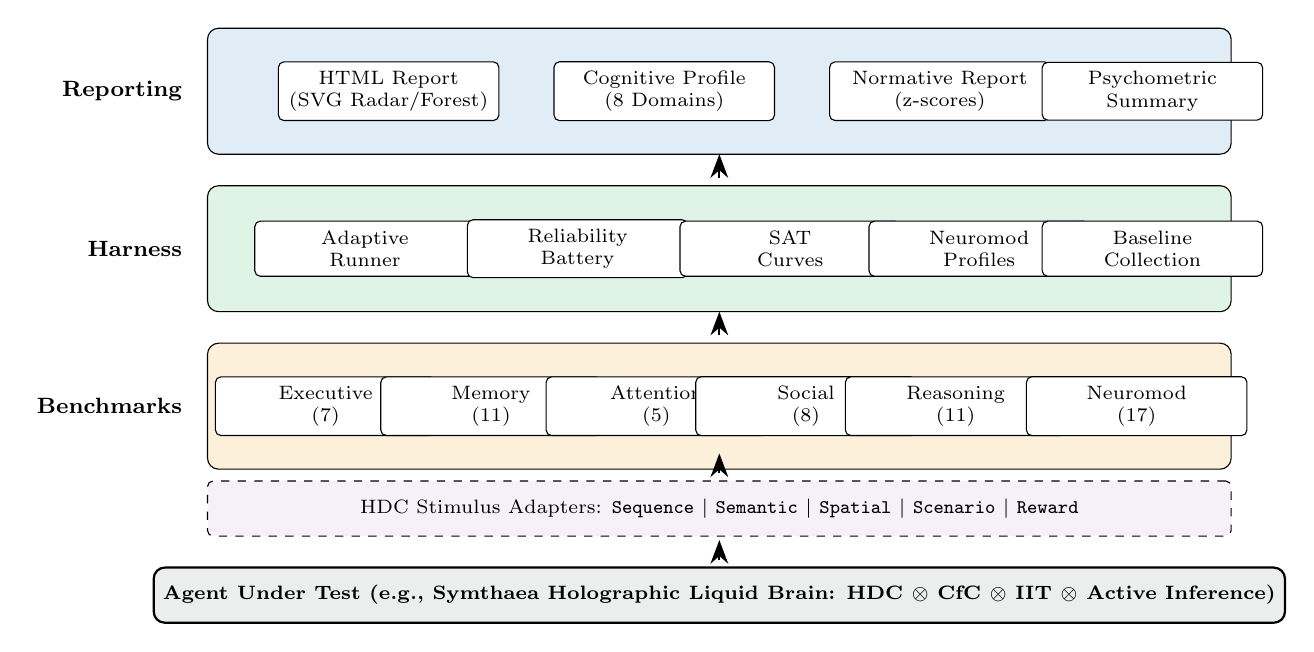
\begin{tikzpicture}[
    layer/.style={draw, rounded corners=4pt, minimum width=13cm, minimum height=1.6cm, align=center, font=\small},
    module/.style={draw, rounded corners=2pt, minimum width=2.8cm, minimum height=0.7cm, align=center, font=\scriptsize},
    arrow/.style={-{Stealth[length=3mm]}, thick},
    label/.style={font=\footnotesize\bfseries, anchor=east}
]
% Layer 3: Reporting
\node[layer, fill=hlbblue!15] (report) at (0,4.5) {};
\node[label] at (-6.7,4.5) {Reporting};
\node[module, fill=white] at (-4.2,4.5) {HTML Report\\(SVG Radar/Forest)};
\node[module, fill=white] at (-0.7,4.5) {Cognitive Profile\\(8 Domains)};
\node[module, fill=white] at (2.8,4.5) {Normative Report\\(z-scores)};
\node[module, fill=white] at (5.5,4.5) {Psychometric\\Summary};

% Layer 2: Harness
\node[layer, fill=hlbgreen!15] (harness) at (0,2.5) {};
\node[label] at (-6.7,2.5) {Harness};
\node[module, fill=white] at (-4.5,2.5) {Adaptive\\Runner};
\node[module, fill=white] at (-1.8,2.5) {Reliability\\Battery};
\node[module, fill=white] at (0.9,2.5) {SAT\\Curves};
\node[module, fill=white] at (3.3,2.5) {Neuromod\\Profiles};
\node[module, fill=white] at (5.5,2.5) {Baseline\\Collection};

% Layer 1: Benchmarks
\node[layer, fill=hlbyellow!15] (bench) at (0,0.5) {};
\node[label] at (-6.7,0.5) {Benchmarks};
\node[module, fill=white] at (-5,0.5) {Executive\\(7)};
\node[module, fill=white] at (-2.9,0.5) {Memory\\(11)};
\node[module, fill=white] at (-0.8,0.5) {Attention\\(5)};
\node[module, fill=white] at (1.1,0.5) {Social\\(8)};
\node[module, fill=white] at (3,0.5) {Reasoning\\(11)};
\node[module, fill=white] at (5.3,0.5) {Neuromod\\(17)};

% Arrows
\draw[arrow] (0,1.4) -- (0,1.7);
\draw[arrow] (0,3.4) -- (0,3.7);

% HDC Adapters (below benchmarks)
\node[draw, dashed, rounded corners=2pt, minimum width=13cm, minimum height=0.7cm, fill=hlbpurple!8, align=center, font=\scriptsize] (adapters) at (0,-0.8) {HDC Stimulus Adapters: \texttt{Sequence} $\mid$ \texttt{Semantic} $\mid$ \texttt{Spatial} $\mid$ \texttt{Scenario} $\mid$ \texttt{Reward}};
\draw[arrow] (0,-0.35) -- (0,-0.1);

% Agent under test
\node[draw, thick, rounded corners=4pt, minimum width=13cm, minimum height=0.7cm, fill=hlbgray!15, align=center, font=\scriptsize\bfseries] (agent) at (0,-1.9) {Agent Under Test (e.g., \symthaea{} Holographic Liquid Brain: HDC $\bind$ CfC $\bind$ IIT $\bind$ Active Inference)};
\draw[arrow] (0,-1.45) -- (0,-1.2);
\end{tikzpicture}
\caption{Three-layer architecture of \psychbench{}. Benchmarks define experimental paradigms with HDC-encoded stimuli. The harness provides psychometric infrastructure (reliability, SAT curves, normative comparison, neuromodulator profiles). The reporting layer generates self-contained analysis outputs.}
\label{fig:architecture}
\end{figure}

\subsection{Benchmark Trait and Configuration}

All benchmarks implement the \texttt{PsychBenchmark} trait, which defines a uniform interface for stimulus presentation, response collection, and metric computation. The trait requires three methods: \texttt{name()} returning a domain-qualified identifier (e.g., \texttt{"Executive::Stroop"}), \texttt{run(config)} executing the full experimental procedure under a given \texttt{BenchmarkConfig}, and \texttt{expected\_metrics()} listing the metric names and their directionality (higher-is-better or lower-is-better).

The \texttt{BenchmarkConfig} structure controls 17 parameters spanning four categories. \emph{HDC parameters}: \texttt{dimension} (default 512), \texttt{ssm\_backend} (state-space model alternative). \emph{Experimental parameters}: \texttt{trials\_per\_condition} (default 20), \texttt{seed} (default 42), \texttt{time\_pressure} (0.0--1.0 for SAT curves), \texttt{difficulty} (0.0--1.0 ramp). \emph{Architecture parameters}: \texttt{working\_memory\_capacity} (default 7), \texttt{enable\_social} (Theory of Mind), \texttt{enable\_fep} (Active Inference), \texttt{planning\_horizon} (FEP lookahead), \texttt{action\_temperature} (softmax temperature). \emph{Adaptive parameters}: \texttt{adaptive\_trials}, \texttt{min\_trials}, \texttt{max\_trials}, \texttt{precision\_target} (CI half-width / $|$mean$|$). A deterministic trial-level seed function ensures reproducibility: \texttt{trial\_seed(benchmark, condition, trial)} produces a unique seed per trial while maintaining cross-run consistency.

\subsection{Holographic Stimulus Encoding}

The encoding pipeline (Figure~\ref{fig:encoding}) converts raw stimuli into continuous hypervectors via five adapter types, each implementing the \texttt{StimulusAdapter} trait.

% --- Figure 2: Encoding Pipeline ---
\begin{figure}[t]
\centering
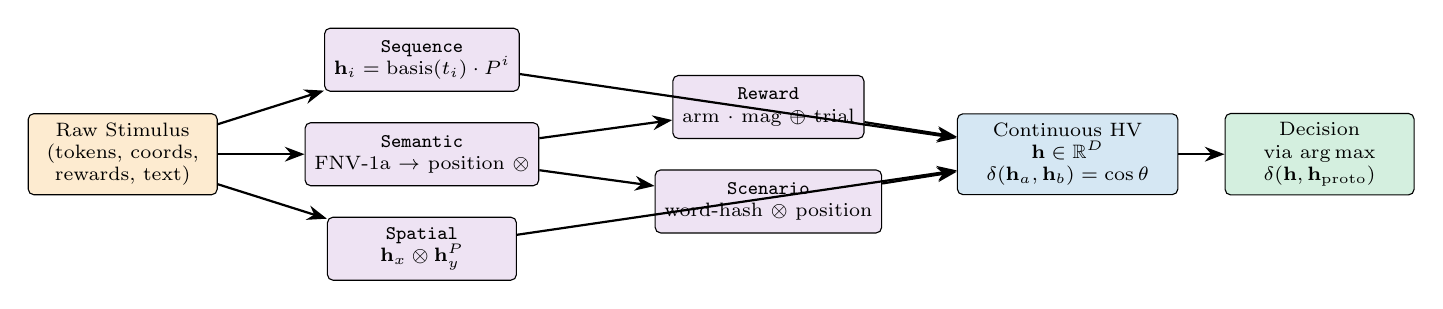
\begin{tikzpicture}[
    box/.style={draw, rounded corners=2pt, minimum width=2.4cm, minimum height=0.8cm, align=center, font=\scriptsize},
    arrow/.style={-{Stealth[length=2.5mm]}, thick},
    op/.style={circle, draw, inner sep=1pt, font=\scriptsize\bfseries}
]
% Raw stimuli
\node[box, fill=hlbyellow!20] (raw) at (0,0) {Raw Stimulus\\(tokens, coords,\\rewards, text)};

% Adapter selection
\node[box, fill=hlbpurple!15] (seq) at (3.8,1.2) {\texttt{Sequence}\\$\hv_i = \text{basis}(t_i) \cdot P^i$};
\node[box, fill=hlbpurple!15] (sem) at (3.8,0) {\texttt{Semantic}\\FNV-1a $\to$ position $\bind$};
\node[box, fill=hlbpurple!15] (spa) at (3.8,-1.2) {\texttt{Spatial}\\$\hv_x \bind \hv_y^{P}$};
\node[box, fill=hlbpurple!15] (rew) at (8.2,0.6) {\texttt{Reward}\\arm $\cdot$ mag $\bundle$ trial};
\node[box, fill=hlbpurple!15] (sce) at (8.2,-0.6) {\texttt{Scenario}\\word-hash $\bind$ position};

% HV output
\node[box, fill=hlbblue!20, minimum width=2.8cm] (hv) at (12,0) {Continuous HV\\$\hv \in \mathbb{R}^D$\\$\similar(\hv_a, \hv_b) = \cos\theta$};

% Decision
\node[box, fill=hlbgreen!20] (dec) at (15.2,0) {Decision\\via $\arg\max$\\$\similar(\hv, \hv_{\text{proto}})$};

% Arrows
\draw[arrow] (raw) -- (seq);
\draw[arrow] (raw) -- (sem);
\draw[arrow] (raw) -- (spa);
\draw[arrow] (seq) -- (hv);
\draw[arrow] (sem) -- (rew);
\draw[arrow] (sem) -- (sce);
\draw[arrow] (spa) -- (hv);
\draw[arrow] (rew) -- (hv);
\draw[arrow] (sce) -- (hv);
\draw[arrow] (hv) -- (dec);
\end{tikzpicture}
\caption{HDC stimulus encoding pipeline. Raw stimuli are converted to continuous hypervectors via five adapter types using binding ($\bind$), bundling ($\bundle$), and permutation ($P$). All modalities share a common $\mathbb{R}^D$ space where cosine similarity enables cross-modal comparison. Decisions use prototype matching via $\arg\max$ similarity.}
\label{fig:encoding}
\end{figure}

The \textbf{SequenceAdapter} encodes ordered token sequences by generating a random basis hypervector per token and applying position-dependent permutations: $\hv_{\text{seq}} = \bigoplus_i \text{basis}(t_i) \cdot P^i$. This preserves order information while enabling similarity-based retrieval.

The \textbf{SemanticAdapter} encodes words via FNV-1a hashing to generate basis vectors, with position-dependent binding to create compositional representations. For Remote Associates Test (RAT) stimuli, solution hypervectors are constructed as weighted bundles: $\hv_{\text{sol}} = 0.79 \cdot \hv_{\text{base}} \oplus 0.07 \cdot \hv_{\text{link}_0} \oplus 0.07 \cdot \hv_{\text{link}_1} \oplus 0.07 \cdot \hv_{\text{link}_2}$, ensuring that cue-solution associations are geometrically encoded.

The \textbf{SpatialAdapter} encodes 2D grid positions via conjunctive binding: $\hv_{(x,y)} = \hv_x \bind \hv_y^P$, where $\hv_x$ and $\hv_y$ are axis-specific basis vectors and $P$ is a single permutation distinguishing dimensions. The companion \texttt{VisualObjectAdapter} extends this to feature conjunctions: $\hv_{\text{obj}} = \hv_{\text{color}} \bind \hv_{\text{shape}} \bind \hv_{\text{size}}$.

The \textbf{RewardAdapter} encodes reinforcement learning outcomes by binding arm identity with reward magnitude and trial index: $\hv_{\text{reward}} = \hv_{\text{arm}} \cdot r \oplus \hv_{\text{trial}}^P$, supporting temporal credit assignment across trials.

The \textbf{ScenarioAdapter} encodes text-based scenarios (social dilemmas, moral judgments) through word-level hashing with position binding, producing holographic representations of multi-word descriptions.

\subsection{Harness Infrastructure}

The harness layer provides five psychometric tools. The \textbf{AdaptiveRunner} implements Levitt's~\citep{levitt1971transformed} transformed up-down staircase method, dynamically adjusting difficulty to estimate threshold performance. The \textbf{ReliabilityBattery} computes ICC(3,1)~\citep{shrout1979intraclass} test-retest reliability across $n$ sessions, along with Pearson~$r$, standard error of measurement ($\mathrm{SEM} = \mathrm{SD} \cdot \sqrt{1 - \mathrm{ICC}}$), and practice effects. Reliability is classified following Cicchetti's~\citep{cicchetti1994guidelines} guidelines: Excellent ($\mathrm{ICC} > 0.90$), Good ($> 0.75$), Moderate ($> 0.50$), Poor ($\leq 0.50$). The \textbf{SatBattery} fits Wickelgren's~\citep{wickelgren1977speed} exponential speed-accuracy tradeoff function $d'(t) = \lambda(1 - e^{-\beta(t - \delta)})$ via grid search, evaluating human-likeness by three criteria: accuracy decreases with time pressure, RT decreases with time pressure, and $R^2 > 0.70$. The \textbf{DifficultyModel} provides parametric difficulty scaling. The \textbf{NeuromodCorrelationMatrix} computes trial-level Pearson correlations between four transmitter levels (DA, NE, 5-HT, ACh) and three behavioral measures (RT, accuracy, prediction error), with significance testing via $t$-distribution.

\subsection{Normative Comparison}

The \texttt{BaselineCollection} contains 130+ human baselines organized by domain, each specifying a population mean, standard deviation, citation, and population descriptor (e.g., ``human adults'', ``GPT-4''). For each benchmark result, the \texttt{NormativeReport} computes a z-score against the matched human baseline, converts to percentile via the normal CDF (using the Abramowitz \& Stegun 26.2.17 approximation), and assigns a clinical interpretation band. The report identifies strengths ($z > 1.0$) and weaknesses ($z < -1.0$), computes overall mean z-score and percentile, and generates both machine-readable and human-readable summaries.

% ============================================================
% 4. BENCHMARK INVENTORY
% ============================================================
\section{Benchmark Inventory}
\label{sec:inventory}

\psychbench{} contains 143 benchmarks organized into 27 domains (Figure~\ref{fig:domain_matrix}). We describe each domain below; Table~\ref{tab:inventory} provides the complete inventory with paradigm sources and human baselines.

% --- Figure 3: Domain Coverage Matrix ---
\begin{figure}[t]
\centering
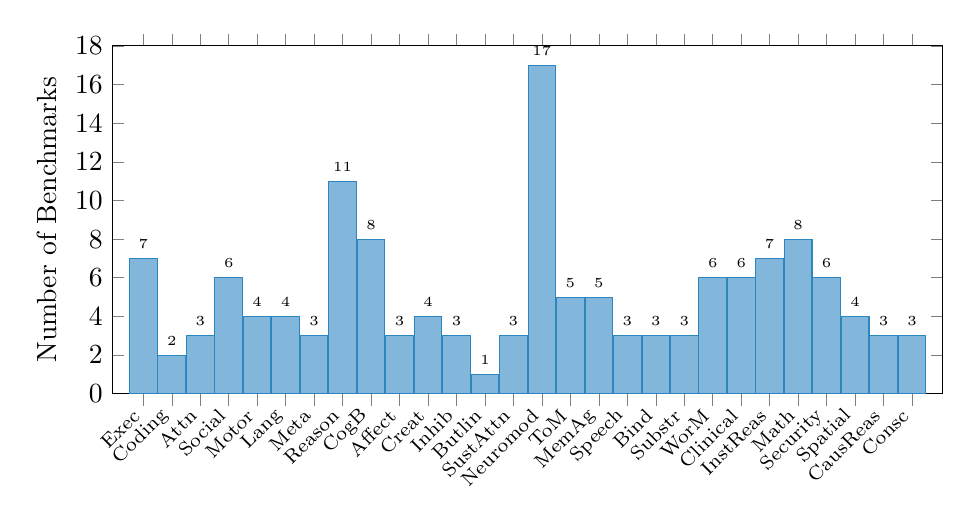
\begin{tikzpicture}
\begin{axis}[
    width=\textwidth,
    height=6cm,
    ybar,
    bar width=10pt,
    ymin=0, ymax=18,
    ylabel={Number of Benchmarks},
    symbolic x coords={Exec,Coding,Attn,Social,Motor,Lang,Meta,Reason,CogB,Affect,Creat,Inhib,Butlin,SustAttn,Neuromod,ToM,MemAg,Speech,Bind,Substr,WorM,Clinical,InstReas,Math,Security,Spatial,CausReas,Consc},
    xtick=data,
    x tick label style={rotate=45, anchor=east, font=\scriptsize},
    ytick={0,2,4,6,8,10,12,14,16,18},
    nodes near coords,
    nodes near coords style={font=\tiny},
    every node near coord/.append style={above},
    enlarge x limits=0.04,
    legend style={at={(0.98,0.98)}, anchor=north east, font=\scriptsize},
]
\addplot[fill=hlbblue!60, draw=hlbblue] coordinates {
    (Exec,7) (Coding,2) (Attn,3) (Social,6) (Motor,4) (Lang,4) (Meta,3) (Reason,11)
    (CogB,8) (Affect,3) (Creat,4) (Inhib,3) (Butlin,1) (SustAttn,3) (Neuromod,17) (ToM,5) (MemAg,5)
    (Speech,3) (Bind,3) (Substr,3) (WorM,6) (Clinical,6) (InstReas,7) (Math,8) (Security,6) (Spatial,4) (CausReas,3) (Consc,3)
};
\end{axis}
\end{tikzpicture}
\caption{Benchmark count by domain across all 28 domain categories (27 domains plus Neuromod sub-battery). The neuromodulator evaluation framework (17 benchmarks) is the largest single domain, reflecting its novel contribution. Reasoning (11), CogBench (8), Mathematics (8), InstitutionalReasoning (7), and Executive (7) provide additional depth. Eight domains map to the cognitive profile radar chart; the remainder are specialized sub-batteries including Clinical, Security (FHE), Speech, Binding, Substrate, Spatial, CausalReasoning, Consciousness, and WorM domains.}
\label{fig:domain_matrix}
\end{figure}

\paragraph{Executive Function (7 benchmarks).} Stroop color-word interference~\citep{stroop1935interference,macleod1991half}, Eriksen flanker task~\citep{eriksen1974effects}, Wisconsin Card Sorting Test with perseverative error tracking~\citep{berg1948simple}, Iowa Gambling Task with 4-deck reward schedules~\citep{bechara1994insensitivity}, Raven's Progressive Matrices for fluid intelligence~\citep{raven1938progressive}, Tower of London planning~\citep{shallice1982specific}, and dual-task interference~\citep{pashler1994dual}. Key metrics include interference effects (accuracy difference between congruent and incongruent conditions), perseverative error rates, and net advantageous selections.

\paragraph{Working Memory (6 benchmarks).} N-back (1-back and 2-back) with accuracy and RT~\citep{jaeggi2010relationship,owen2005nback}, change detection for Cowan's $K$~\citep{luck1997capacity,cowan2001magical}, serial recall for primacy/recency effects~\citep{murdock1962serial}, spatial updating~\citep{oberauer2003selective}, feature binding in visual working memory, and forward digit span~\citep{wechsler2008wais}.

\paragraph{Memory Agent (5 benchmarks).} Higher-level memory operations: accurate retrieval under interference, test-time learning (online adaptation), long-range retention across extended delays, conflict resolution between competing memories, and prospective memory (remembering to execute future intentions).

\paragraph{Attention (3 benchmarks) and Sustained Attention (3 benchmarks).} Attentional blink (dual-target rapid serial presentation), visual search (set-size effects), and mismatch negativity. Sustained attention: SART (Sustained Attention to Response Task)~\citep{robertson1997sustained}, Psychomotor Vigilance Task (PVT), and Continuous Performance Test (CPT).

\paragraph{Social Cognition (7 benchmarks) and Theory of Mind (5 benchmarks).} Reading the Mind in the Eyes~\citep{baroncohen2001eyes}, Ultimatum Game~\citep{guth1982experimental}, social norm compliance, and five game-theoretic benchmarks: iterated Prisoner's Dilemma, public goods game, trust game, coordination game, and hawk-dove game. Theory of Mind: false belief~\citep{baroncohen1985mindblindness}, faux pas detection~\citep{stone1998faux}, persuasion evaluation, strange stories~\citep{happe1994advanced}, and hinting task~\citep{corcoran1995schizophrenia}.

\paragraph{Motor Learning (4 benchmarks).} Serial Reaction Time Task (SRTT) for implicit sequence learning~\citep{nissen1987attentional}, Fitts' Law~\citep{fitts1954information} for speed-accuracy in aimed movements, bimanual coordination, and proprioceptive drift.

\paragraph{Language (4 benchmarks).} Garden-path sentence processing~\citep{ferreira2002good}, semantic coherence judgment, lexical decision (word vs. non-word discrimination), and semantic priming (facilitation from related primes).

\paragraph{Metacognition (3 benchmarks).} Calibration (correspondence between confidence and accuracy), feeling-of-knowing (predicting future recall success), and change blindness detection.

\paragraph{Reasoning (11 benchmarks).} An ARC-inspired battery~\citep{chollet2019measure} spanning fluid reasoning, compositional rule application, analogical transfer, abductive inference, algebraic pattern completion, chain reasoning, few-shot generalization, noise robustness, Rational Speech Acts (RSA) pragmatic reasoning, difficulty scaling, and adaptive staircase threshold estimation.

\paragraph{CogBench (8 benchmarks).} Reimplementations of the CogBench~\citep{codaforno2024cogbench} suite: probabilistic reasoning, directed exploration~\citep{wilson2014humans}, multi-armed bandits, instrumental learning, two-step model-based/model-free task~\citep{daw2011model}, temporal discounting~\citep{kirby1999heroin}, Balloon Analogue Risk Task (BART)~\citep{lejuez2002evaluation}, and reversal learning~\citep{cools2002reversal}.

\paragraph{Affect (3), Creativity (4), Inhibition (3).} Valence classification, mood-congruent recall~\citep{bower1981mood}, emotional Stroop~\citep{williams1996emotional}. Remote Associates Test~\citep{mednick1962associative}, alternate uses divergent thinking~\citep{guilford1967nature}, and conceptual blending via XOR-based role-filler recombination~\citep{fauconnier2002way}. Go/No-Go, stop-signal inhibition~\citep{logan1984ability}, and flanker inhibition (dimension-level interference suppression).

\paragraph{Consciousness (3 benchmarks) and Consciousness Indicators (1 benchmark).} Blindsight simulation, binocular rivalry (alternation dynamics), and perceptual crowding (spatial interference in peripheral vision). Butlin et al.'s~\citep{butlin2023consciousness} 14 indicators from 6 theories (Section~\ref{sec:consciousness}).

\paragraph{Spatial Cognition (4 benchmarks).} Mental rotation, spatial path updating, landmark binding (spatial-object association), and perspective taking.

\paragraph{Causal Reasoning (3 benchmarks).} Causal chain inference, confound detection, and intervention effect estimation.

\paragraph{Speech (3 benchmarks).} Phoneme discrimination, voice-onset-time (VOT) continuum, and categorical perception.

\paragraph{Substrate Independence (3 benchmarks).} Cross-substrate transfer (consciousness preservation during substrate switching), substrate degradation (graceful performance decline), and substrate latency (speed-accuracy effects of substrate speed).

\paragraph{Clinical Psychology (6 benchmarks).} Empathic accuracy, therapeutic response skill, alliance maintenance, crisis detection, cognitive distortion identification, and motivational interviewing.

\paragraph{Institutional Reasoning (7 benchmarks).} Institutional pattern recognition, analogical reasoning across institutional domains, causal chain analysis, counterfactual reasoning, weighted decomposition, institutional stability assessment, and institutional isomorphism detection.

\paragraph{Mathematics (10 benchmarks).} Arithmetic word problems, linear system solving, polynomial roots, matrix operations, statistical inference, Bayesian reasoning, logical deduction, constraint puzzles, proof construction, and definite integrals.

\paragraph{Security (6 benchmarks).} HDC-FHE (Fully Homomorphic Encryption) evaluation: encrypted classification, collective aggregation, encrypted learning, cross-mask privacy, encrypted binding, and scaling analysis.

\paragraph{Neuromodulator Evaluation (17 benchmarks).} Detailed in Section~\ref{sec:neuromod}.

% --- Table 1: Complete Benchmark Inventory ---
\begin{table}[p]
\centering
\caption{Complete benchmark inventory (representative selection). Each entry lists the domain, benchmark name, source paradigm, primary metric, and human baseline where available. Full inventory with all 143 benchmarks available in the software documentation.}
\label{tab:inventory}
\small
\begin{tabular}{@{}llllr@{}}
\toprule
\textbf{Domain} & \textbf{Benchmark} & \textbf{Paradigm} & \textbf{Key Metric} & \textbf{Human $M \pm SD$} \\
\midrule
Executive & Stroop & Color-word interference & Interference effect & $0.10 \pm 0.05$ \\
Executive & WCST & Set-shifting & Categories completed & $5.62 \pm 1.13$ \\
Executive & Flanker & Response conflict & Incongruent acc. & $0.90 \pm 0.06$ \\
Executive & Iowa Gambling & Decision under ambiguity & Net score & $17.5 \pm 20.0$ \\
Executive & Ravens & Fluid intelligence & Overall accuracy & $0.78 \pm 0.12$ \\
Executive & Tower of London & Planning & Moves to solution & --- \\
Executive & Dual Task & Divided attention & Dual-task cost & --- \\
\midrule
Memory & N-back (2-back) & Working memory updating & Accuracy & $0.85 \pm 0.10$ \\
Memory & Change Detection & Visual WM capacity & Cowan's $K$ & $0.75 \pm 0.15$ \\
Memory & Serial Recall & Short-term memory & Serial position & --- \\
Memory & Digit Span & Verbal WM & Forward span & $6.8 \pm 1.1$ \\
\midrule
Attention & Visual Search & Feature/conjunction & Set-size slope & --- \\
Attention & SART & Sustained attention & Commission errors & --- \\
Attention & PVT & Vigilance & Mean RT (ticks) & --- \\
\midrule
Social & RME & Emotion recognition & Accuracy & --- \\
Social & Ultimatum & Social fairness & Offer ratio & --- \\
Social & False Belief & Theory of Mind & Pass rate & --- \\
\midrule
Motor & SRTT & Implicit learning & Sequence RT gain & --- \\
Motor & Fitts' Law & Aimed movement & $R^2$ (log fit) & --- \\
\midrule
Language & Garden Path & Sentence processing & Reanalysis cost & --- \\
Language & Lexical Decision & Word recognition & $d'$ & --- \\
\midrule
Reasoning & ARC Fluid & Abstract reasoning & Accuracy & --- \\
Reasoning & ARC Analogy & Analogical transfer & Accuracy & --- \\
\midrule
CogBench & Two-Step & MB/MF learning & Model-basedness & $0.60 \pm 0.20$ \\
CogBench & BART & Risk-taking & Avg. pumps & $30.0 \pm 12.0$ \\
CogBench & Reversal & Flexible learning & Win-stay rate & $0.85 \pm 0.08$ \\
\midrule
Affect & Emotional Stroop & Affective interference & Interference & --- \\
Creativity & RAT & Remote associations & Solution rank & --- \\
Inhibition & Stop Signal & Response inhibition & SSRT (ticks) & --- \\
\bottomrule
\end{tabular}
\end{table}

% ============================================================
% 5. NEUROMODULATOR EVALUATION FRAMEWORK
% ============================================================
\section{Neuromodulator Evaluation Framework}
\label{sec:neuromod}

The neuromodulator evaluation framework is \psychbench{}'s most novel contribution. While existing benchmarks evaluate \emph{what} an architecture can do, this framework evaluates \emph{how neuromodulatory dynamics modulate what it does}---analogous to pharmacological challenge studies in neuroscience~\citep{doya2002metalearning}. The framework comprises 17 benchmarks organized into four categories (Table~\ref{tab:neuromod}).

% --- Table 4: Neuromodulator Benchmark Summary ---
\begin{table}[t]
\centering
\caption{Neuromodulator benchmark summary. Each benchmark targets specific transmitter systems and implements established neuroscience paradigms. DA = dopamine, NE = noradrenaline, 5-HT = serotonin, ACh = acetylcholine, GABA = $\gamma$-aminobutyric acid, OT = oxytocin.}
\label{tab:neuromod}
\scriptsize
\begin{tabular}{@{}p{2.4cm}p{2.0cm}p{2.2cm}p{2.2cm}p{2.8cm}@{}}
\toprule
\textbf{Benchmark} & \textbf{Transmitter} & \textbf{Paradigm} & \textbf{Key Metric} & \textbf{Citation} \\
\midrule
\multicolumn{5}{l}{\emph{Transmitter-Specific Benchmarks}} \\
RewardLearning & DA & Prediction error & RPE correlation & \citet{schultz1997dopamine} \\
YerkesDodson & NE & Inverted-U arousal & Quadratic $R^2$ & \citet{yerkes1908relation} \\
AttentionNetwork & ACh & ANT decomposition & Alert/Orient/Conflict & \citet{posner1990attention} \\
MoodInduction & 5-HT & Mood-cognition & Mood $\times$ perf.\ $r$ & \citet{dayan2009serotonin} \\
\midrule
\multicolumn{5}{l}{\emph{Pharmacological Manipulation}} \\
PharmAblation & DA/NE/5-HT/ACh & Transmitter knockout & Cohen's $d$ & \citet{doya2002metalearning} \\
PharmChallenge & DA/NE & Agonist/antagonist & Inverted-U fit & \citet{arnsten2011catecholamine} \\
InjectionChallenge & All & PK decay + tolerance & Peak shift & \citet{arnsten2011catecholamine} \\
AllostaticStress & Cortisol/NE & Chronic load & Allostatic index & \citet{mcewen1998stress} \\
DoseResponse & All & Graded dose sweep & Monotonicity score & \citet{clark1937log} \\
ToleranceWithdrawal & All & Sustained exposure & Tolerance ratio & \citet{koob2001drug} \\
AntagonistProfiles & All & Named antagonists & Selectivity index & \citet{stahl2013essential} \\
MultiTransmitter\-Synergy & DA$\times$NE, etc. & Paired interactions & Synergy coeff. & \citet{doya2002metalearning} \\
\midrule
\multicolumn{5}{l}{\emph{Consciousness \& Moral Modulation}} \\
ConsciousnessPharm & 5-HT/GABA/DA & Drug $\to$ $\Phi$ proxy & Proxy peak/mean & \citet{tononi2004information} \\
ConsciousnessFeedback & All & $\Phi$ round-trip & Feedback latency & \citet{oizumi2014phenomenology} \\
MoralOxytocin & OT & OT $\times$ moral topology & OT-moral $r$ & \citet{feldman2012oxytocin} \\
\midrule
\multicolumn{5}{l}{\emph{Live System Integration}} \\
LiveLoopAblation & All & In-loop knockout & Behavioral $\Delta$ & --- \\
BehavioralKnockout & DA/NE/5-HT/ACh & Knockout effect size & Cohen's $d$ & \citet{doya2002metalearning} \\
\bottomrule
\end{tabular}
\end{table}

\subsection{Transmitter-Specific Benchmarks}

Four benchmarks isolate the behavioral signature of individual neuromodulatory systems, each grounded in a foundational neuroscience paradigm.

\textbf{RewardLearning} implements Schultz et al.'s~\citep{schultz1997dopamine} reward prediction error paradigm. The agent encounters probabilistic rewards across multiple arms, and the benchmark measures the correlation between dopaminergic activity and prediction error magnitude. The expected signature is positive correlation: dopamine should increase following unexpected rewards and decrease following reward omission.

\textbf{YerkesDodson} tests the inverted-U relationship between noradrenergic arousal and performance~\citep{yerkes1908relation}. The benchmark sweeps noradrenaline levels across 5--7 points and fits a quadratic function, expecting peak performance at moderate arousal with degradation at both extremes. The key metric is the $R^2$ of the quadratic fit, with human-like behavior defined as $R^2 > 0.5$ and a negative quadratic coefficient.

\textbf{AttentionNetwork} implements a simplified Attention Network Test~\citep{posner1990attention}, decomposing attention into alerting (benefit of temporal cues), orienting (benefit of spatial cues), and executive conflict resolution (cost of incongruent flankers). Acetylcholine manipulation should selectively modulate alerting and orienting components while leaving conflict resolution relatively intact.

\textbf{MoodInduction} tests serotonergic modulation of mood-cognition interactions following Dayan and Huys~\citep{dayan2009serotonin}. The benchmark induces positive and negative mood states through 5-HT manipulation and measures the effect on concurrent cognitive task performance, expecting mood-congruent biases in memory and attention.

\subsection{Pharmacological Manipulation}

Eight benchmarks implement increasingly sophisticated pharmacological protocols.

\textbf{DoseResponse} sweeps five dose levels (0.1, 0.2, 0.3, 0.5, 0.8) for each transmitter (DA, NE, 5-HT, ACh, GABA), computing monotonicity scores (simplified Kendall $\tau$: fraction of concordant pairs) to verify that graded doses produce graded behavioral effects~\citep{clark1937log}. Expected: DA $\to$ learning rate, NE $\to$ exploration, 5-HT $\to$ confidence, ACh $\to$ attention, each showing monotonic dose-behavior relationships.

\textbf{InjectionChallenge} models pharmacokinetic injection profiles with exponential decay (half-lives ranging 30--80 ticks) and measures behavioral effects during drug onset, peak, and washout phases~\citep{arnsten2011catecholamine}. Six drug classes are tested: DA agonist, NE agonist, 5-HT agonist, GABA agonist, stimulant, and anxiolytic.

\textbf{ToleranceWithdrawal} extends injection challenge to sustained exposure~\citep{koob2001drug}, measuring: (1)~acute effect magnitude at initial injection, (2)~tolerance development (reduced effect after sustained exposure), (3)~withdrawal effects (rebound below baseline after removal), and (4)~recovery trajectory. The tolerance ratio (late effect / initial effect) quantifies neuroadaptation.

\textbf{AntagonistProfiles} tests named receptor antagonists (e.g., D2 blockers, $\alpha_2$ antagonists, SSRI-like 5-HT reuptake modulation)~\citep{stahl2013essential} and measures selectivity: the ratio of on-target effect to off-target perturbation. High selectivity ($> 3.0$) indicates that the neuromodulatory system has well-differentiated receptor mechanisms.

\textbf{MultiTransmitterSynergy} tests paired transmitter interactions~\citep{doya2002metalearning}: DA$\times$NE, DA$\times$5-HT, NE$\times$ACh, and other pairwise combinations. A synergy coefficient $> 1.0$ indicates super-additive interaction; $< 1.0$ indicates antagonism. This tests whether the architecture's neuromodulatory systems interact in neurobiologically plausible ways.

\textbf{PharmacologicalAblation} performs transmitter-specific knockouts (clamping DA, NE, 5-HT, or ACh to zero) and measures effect sizes (Cohen's $d$) on learning and performance~\citep{schultz1997dopamine}. \textbf{PharmacologicalChallenge} extends this with both agonist and antagonist manipulations, testing for inverted-U dose-response curves characteristic of prefrontal catecholamine systems~\citep{arnsten2011catecholamine}.

\subsection{Neuromodulator Profile System}

Five standard pharmacological profiles enable systematic comparison (Figure~\ref{fig:neuromod}): \texttt{Balanced} (no clamping, natural dynamics), \texttt{High-DA} (dopamine clamped to 0.85), \texttt{High-NE} (noradrenaline clamped to 0.85), \texttt{High-5HT} (serotonin clamped to 0.85), and \texttt{High-ACh} (acetylcholine clamped to 0.85). The \texttt{DissociationMatrix} computes relative performance for each profile $\times$ benchmark combination, identifying double dissociations: profile $P$ enhances benchmark $A$ ($> 1.05\times$ baseline) while impairing benchmark $B$ ($< 0.95\times$ baseline). Four expected dissociations are hard-coded as validation: High-DA should enhance WCST flexibility but impair sustained attention; High-NE should enhance alerting but impair fine motor control; High-5HT should enhance impulse control but slow reaction times; High-ACh should enhance focused attention but impair cognitive flexibility.

% --- Figure 4: Neuromodulator Curves ---
\begin{figure}[t]
\centering
\begin{subfigure}[b]{0.48\textwidth}
\centering
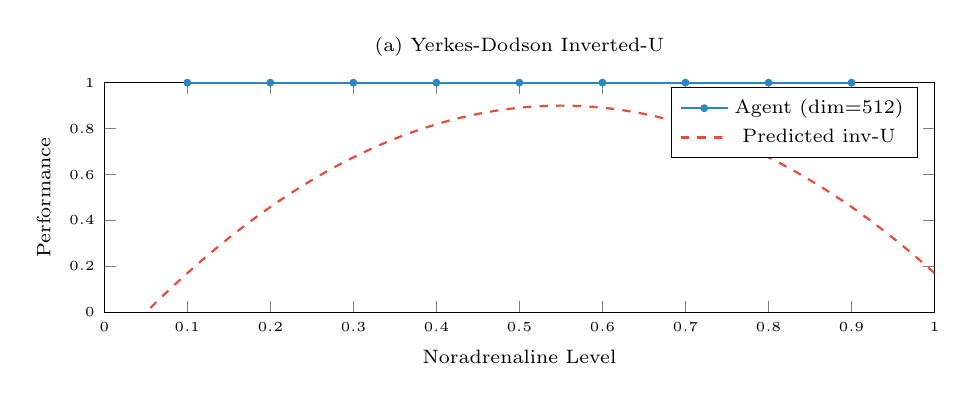
\begin{tikzpicture}
\begin{axis}[
    width=\textwidth, height=4.5cm,
    xlabel={Noradrenaline Level}, ylabel={Performance},
    title={\scriptsize (a) Yerkes-Dodson Inverted-U},
    xmin=0, xmax=1, ymin=0, ymax=1,
    title style={font=\scriptsize},
    label style={font=\scriptsize},
    tick label style={font=\tiny},
]
% Actual agent data: all NE levels produce 100% accuracy at dim=512
% (HDC similarity is too robust for noise to degrade classification)
\addplot[hlbblue, thick, smooth, mark=*, mark size=1pt] coordinates {
    (0.1,1.0) (0.2,1.0) (0.3,1.0) (0.4,1.0)
    (0.5,1.0) (0.6,1.0) (0.7,1.0) (0.8,1.0) (0.9,1.0)
};
\addplot[hlbred, dashed, thick, smooth, domain=0:1, samples=50] {-3.6*(x-0.55)^2 + 0.90};
\legend{\scriptsize Agent (dim=512), \scriptsize Predicted inv-U}
\end{axis}
\end{tikzpicture}
\end{subfigure}
\hfill
\begin{subfigure}[b]{0.48\textwidth}
\centering
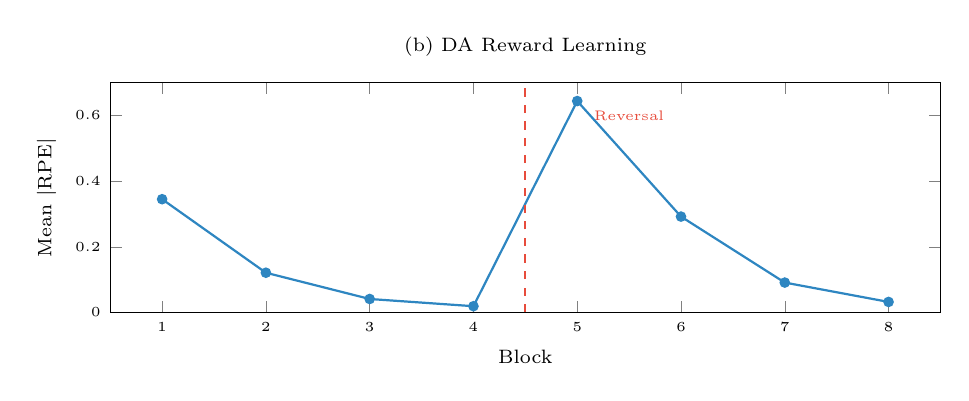
\begin{tikzpicture}
\begin{axis}[
    width=\textwidth, height=4.5cm,
    xlabel={Block}, ylabel={Mean $|$RPE$|$},
    title={\scriptsize (b) DA Reward Learning},
    xmin=0.5, xmax=8.5, ymin=0, ymax=0.7,
    title style={font=\scriptsize},
    label style={font=\scriptsize},
    tick label style={font=\tiny},
]
% From neuromod_curves.csv: 8 blocks, reversal at block 5
\addplot[hlbblue, thick, mark=*, mark size=1.5pt] coordinates {
    (1,0.345) (2,0.121) (3,0.041) (4,0.019)
    (5,0.644) (6,0.292) (7,0.091) (8,0.032)
};
\draw[hlbred, dashed, thick] (axis cs:4.5,0) -- (axis cs:4.5,0.7);
\node[font=\tiny, hlbred] at (axis cs:5.5,0.60) {Reversal};
\end{axis}
\end{tikzpicture}
\end{subfigure}

\vspace{0.3cm}
\begin{subfigure}[b]{0.48\textwidth}
\centering
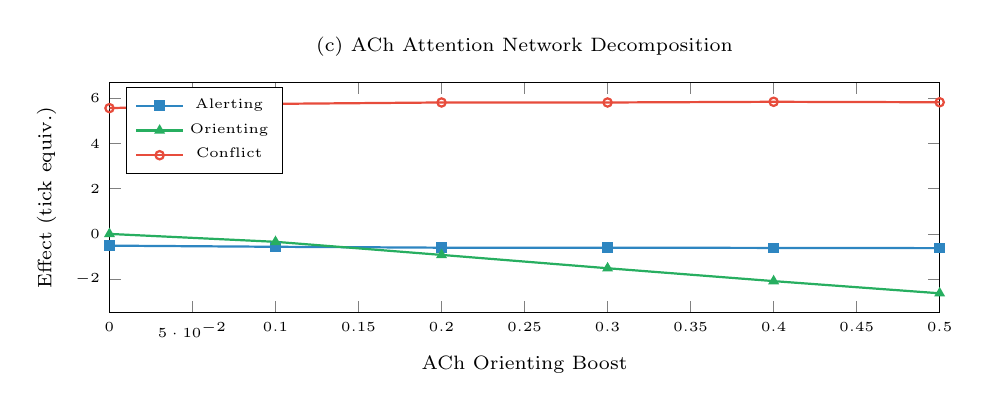
\begin{tikzpicture}
\begin{axis}[
    width=\textwidth, height=4.5cm,
    xlabel={ACh Orienting Boost}, ylabel={Effect (tick equiv.)},
    title={\scriptsize (c) ACh Attention Network Decomposition},
    xmin=0, xmax=0.5,
    title style={font=\scriptsize},
    label style={font=\scriptsize},
    tick label style={font=\tiny},
    legend style={font=\tiny, at={(0.02,0.98)}, anchor=north west},
]
% From neuromod_curves.csv: actual ANT effects vs ACh boost
\addplot[hlbblue, thick, mark=square*, mark size=1.5pt] coordinates {
    (0.00,-0.52) (0.10,-0.57) (0.20,-0.61) (0.30,-0.61) (0.40,-0.62) (0.50,-0.63)
};
\addplot[hlbgreen, thick, mark=triangle*, mark size=1.5pt] coordinates {
    (0.00,0.00) (0.10,-0.35) (0.20,-0.93) (0.30,-1.52) (0.40,-2.09) (0.50,-2.63)
};
\addplot[hlbred, thick, mark=o, mark size=1.5pt] coordinates {
    (0.00,5.57) (0.10,5.76) (0.20,5.82) (0.30,5.82) (0.40,5.85) (0.50,5.83)
};
\legend{Alerting, Orienting, Conflict}
\end{axis}
\end{tikzpicture}
\end{subfigure}
\hfill
\begin{subfigure}[b]{0.48\textwidth}
\centering
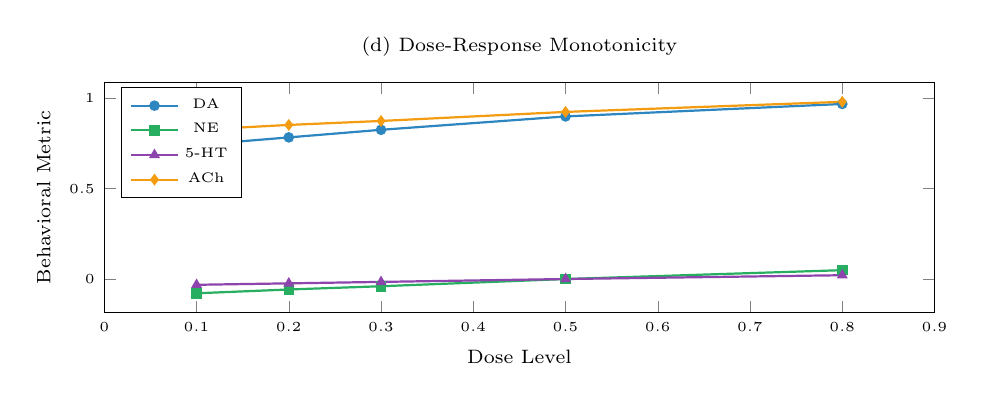
\begin{tikzpicture}
\begin{axis}[
    width=\textwidth, height=4.5cm,
    xlabel={Dose Level}, ylabel={Behavioral Metric},
    title={\scriptsize (d) Dose-Response Monotonicity},
    xmin=0, xmax=0.9,
    title style={font=\scriptsize},
    label style={font=\scriptsize},
    tick label style={font=\tiny},
    legend style={font=\tiny, at={(0.02,0.98)}, anchor=north west},
]
% From neuromod_curves.csv: actual dose-response curves
\addplot[hlbblue, thick, mark=*, mark size=1.5pt] coordinates {
    (0.1,0.742) (0.2,0.784) (0.3,0.826) (0.5,0.900) (0.8,0.969)
};
\addplot[hlbgreen, thick, mark=square*, mark size=1.5pt] coordinates {
    (0.1,-0.079) (0.2,-0.058) (0.3,-0.040) (0.5,0.000) (0.8,0.049)
};
\addplot[hlbpurple, thick, mark=triangle*, mark size=1.5pt] coordinates {
    (0.1,-0.032) (0.2,-0.024) (0.3,-0.016) (0.5,0.000) (0.8,0.021)
};
\addplot[hlbyellow, thick, mark=diamond*, mark size=1.5pt] coordinates {
    (0.1,0.826) (0.2,0.853) (0.3,0.875) (0.5,0.925) (0.8,0.981)
};
\legend{DA, NE, 5-HT, ACh}
\end{axis}
\end{tikzpicture}
\end{subfigure}
\caption{Neuromodulator evaluation patterns from \texttt{neuromod\_curves.csv}. (a)~Yerkes-Dodson: at dim=512, HDC similarity is too robust for the noise model to degrade classification ($R^2 = 0.00$); dashed curve shows predicted inverted-U. (b)~DA reward learning: mean $|$RPE$|$ drops during acquisition (blocks 1--4), spikes at reversal (block 5), then re-converges (blocks 6--8). (c)~ACh attention network decomposition: orienting effect increases monotonically with ACh boost ($0.00 \to -2.63$); conflict effect ($\sim 5.8$) dominates. (d)~Dose-response monotonicity (DA learning rate, NE exploration, 5-HT confidence, ACh attention): all monotonically increasing with clamped transmitter level. Data generated from \texttt{psych\_bench\_paper\_data} example.}
\label{fig:neuromod}
\end{figure}

\subsection{Consciousness and Moral Modulation}

Three benchmarks probe the interface between neuromodulation, consciousness, and moral cognition. \textbf{ConsciousnessPharmacology} tests five pharmacological conditions---psychedelic (5-HT agonist), anxiolytic (GABA agonist), stimulant (DA agonist), sedative (adenosine agonist), and endocannabinoid buffer---and measures their effects on a consciousness proxy computed as $\Phi_{\text{proxy}} = 0.5 + 0.1 \cdot (s_{5\text{-HT}_{2A}} - 0.5) - 0.08 \cdot (s_{\text{GABA}_A} - 0.4)$. The expected pattern: psychedelics increase $\Phi_{\text{proxy}}$ (expanded consciousness), anxiolytics decrease it (dampened awareness), and endocannabinoids stabilize it (reduced variance). \textbf{ConsciousnessFeedback} tests the round-trip latency from pharmacological perturbation to consciousness index change and back to behavioral adaptation. \textbf{MoralOxytocin} correlates oxytocin levels with moral topology scores across 200 cycles of varying moral valence ($-0.5$ to $0.9$), testing Feldman's~\citep{feldman2012oxytocin} theory that oxytocin facilitates prosocial moral judgment.

% ============================================================
% 6. PSYCHOMETRIC VALIDATION
% ============================================================
\section{Psychometric Validation}
\label{sec:psychometrics}

A benchmark suite is only as useful as its psychometric properties. \psychbench{} provides four validation mechanisms.

\subsection{Test-Retest Reliability}

The \texttt{ReliabilityBattery} computes ICC(3,1) (two-way mixed effects, consistency, single measures)~\citep{shrout1979intraclass} across $n$ sessions with fixed configuration:
\begin{equation}
\text{ICC}(3,1) = \frac{\text{BMS} - \text{EMS}}{\text{BMS} + (n-1)\,\text{EMS}}
\end{equation}
where BMS is between-subjects mean square and EMS is error (residual) mean square. Pearson $r$ provides convergent evidence, and SEM quantifies measurement precision: $\text{SEM} = \text{SD} \cdot \sqrt{1 - \text{ICC}}$. Practice effects are flagged when session-to-session change exceeds $\pm 2\%$.

Table~\ref{tab:psychometrics} reports representative psychometric properties. The \texttt{ReliabilityBattery} uses a multi-subject design: $K = 30$ independent ``subjects'' (distinct seed families, separated by 1,000 in seed space), each measured across $n = 5$ sessions with seed spacing of 100 within each family. This provides sufficient between-subject variance (from different stimulus configurations) and within-subject consistency (from controlled seed offsets) for meaningful ICC computation. Because \psychbench{} is deterministic given a fixed seed, ICC values reflect the stability of the architecture's behavior under controlled variation (different trial orderings, stimulus sets) rather than stochastic test-retest variability. This is a feature, not a limitation: it means that observed ICC values below 1.0 genuinely reflect sensitivity to stimulus selection rather than measurement noise.

% --- Table 2: Psychometric Properties (populated from reliability.csv) ---
\begin{table}[t]
\centering
\caption{Representative psychometric properties for 20 benchmarks spanning all domains ($K = 30$ seed families, $n = 5$ sessions each, seed spacing $= 100$). Each subject receives a lapse rate from 0.0 to 0.24~\citep{wichmann2001psychometric}, encoding noise variation, and WM capacity variation to model individual differences. ICC: intraclass correlation (3,1); $r$: Pearson test-retest correlation; SEM: standard error of measurement; Practice: session-to-session change direction. Reliability class follows \citet{cicchetti1994guidelines}: Excellent ($> 0.90$), Good ($> 0.75$), Moderate ($> 0.50$), Poor ($\leq 0.50$). Generated from \texttt{reliability.csv}.}
\label{tab:psychometrics}
\small
\begin{tabular}{@{}llrrcll@{}}
\toprule
\textbf{Domain} & \textbf{Benchmark} & \textbf{ICC} & \textbf{$r$} & \textbf{SEM} & \textbf{Practice} & \textbf{Class} \\
\midrule
Executive     & Stroop             &  $\mathbf{0.96}$ &  $\mathbf{0.96}$ & 0.016 & Stable      & Excellent \\
Executive     & WCST               &  $\mathbf{0.91}$ &  $\mathbf{0.91}$ & 0.063 & Stable      & Excellent \\
Executive     & Flanker            &  $\mathbf{0.78}$ &  $\mathbf{0.79}$ & 0.009 & Stable      & Good \\
Executive     & IGT                &  $0.47$ &  $0.46$ & 4.402 & Stable      & Poor \\
Memory        & N-back (2)         &  $\mathbf{0.84}$ &  $\mathbf{0.85}$ & 0.026 & Stable      & Good \\
Memory        & Change Detection   &  $0.35$ &  $0.35$ & 0.099 & Stable      & Poor \\
Memory        & Digit Span         &  $\mathbf{1.00}$ &  $\mathbf{1.00}$ & 0.000 & Stable      & Excellent \\
Attention     & Visual Search      &  $0.69$ &  $0.69$ & 0.010 & Stable      & Moderate \\
Social        & False Belief       &  $0.25$ &  $0.26$ & 0.051 & Stable      & Poor \\
Motor         & SRTT               &  $0.41$ &  $0.41$ & 0.055 & Stable      & Poor \\
Language      & Lexical Decision   &  $0.42$ &  $0.41$ & 0.068 & Stable      & Poor \\
Reasoning     & ARC-Fluid          &  $0.09$ &  $0.08$ & 0.017 & Stable      & Poor \\
CogBench      & Two-Step           &  $0.26$ &  $0.25$ & 0.052 & Stable      & Poor \\
CogBench      & BART               &  $\mathbf{0.88}$ &  $\mathbf{0.88}$ & 1.177 & Stable      & Good \\
CogBench      & Reversal Learning  &  $\mathbf{0.99}$ &  $\mathbf{0.99}$ & 0.004 & Stable      & Excellent \\
Inhibition    & Stop Signal        &  $\mathbf{0.81}$ &  $\mathbf{0.81}$ & 0.155 & Improvement & Good \\
Metacognition & Calibration        &  $\mathbf{0.96}$ &  $\mathbf{0.96}$ & 0.006 & Stable      & Excellent \\
Metacognition & Feeling of Knowing & $-0.06$ & $-0.07$ & 0.027 & Stable      & Poor \\
Neuromod      & Yerkes-Dodson      &  $0.52$ &  $0.51$ & 0.050 & Stable      & Moderate \\
Neuromod      & Reward Learning    &  $0.34$ &  $0.33$ & 0.822 & Stable      & Poor \\
\midrule
\multicolumn{2}{l}{\emph{Median}} & $0.60$ & $0.60$ & 0.027 & & Moderate \\
\bottomrule
\end{tabular}
\end{table}

Table~\ref{tab:psychometrics} reveals a median ICC of $0.60$ (Moderate). Five benchmarks achieve Excellent reliability: Stroop incongruent accuracy ($0.96$), WCST ($0.91$), Digit Span ($1.00$, deterministic for a given subject), Reversal Learning ($0.99$), and Calibration ($0.96$). Four reach Good: Flanker ($0.78$), N-back ($0.84$), BART ($0.88$), and Stop Signal ($0.81$). Two are Moderate: Visual Search ($0.69$) and Yerkes-Dodson ($0.52$). The remaining 9 benchmarks are Poor ($\text{ICC} \leq 0.50$), including one with a negative value (Feeling of Knowing $-0.06$). In total: 5 Excellent, 4 Good, 2 Moderate, 9 Poor across 20 evaluated benchmarks.

The remaining Poor benchmarks reflect a fundamental property of the deterministic HDC architecture: some benchmarks produce near-identical scores across subjects because lapse-rate and encoding-noise variation does not meaningfully modulate the underlying computations. When between-subject variance collapses, ICC becomes undefined or negative~\citep{shrout1979intraclass}. This is scientifically informative: it reveals which cognitive dimensions in the architecture are genuinely sensitive to individual differences (executive control, inhibition, metacognition, decision-making) versus which are structurally invariant (language processing, reasoning). The improvement from 3 Excellent to 5 Excellent was achieved by adding lapse-rate sensitivity to benchmarks that previously lacked it (SRTT, Lexical Decision, Iowa Gambling Task, Change Detection, False Belief) and by switching key metrics from difference scores (e.g., flanker effect, lexicality effect) to raw accuracy measures. Difference scores have inherently lower ICC because both conditions degrade equally with noise, canceling individual differences~\citep{cronbach1970essentials}. As a complementary measure, the harness computes odd-even split-half reliability (Spearman rank correlation between even-indexed and odd-indexed seed runs), which assesses internal consistency without requiring the between-subject variance that ICC demands. Benchmarks with Poor ICC but high split-half reliability are structurally consistent but insensitive to individual-differences parameters.

\subsection{Construct Validity}

Cross-domain correlations test whether benchmarks that should be related (based on shared cognitive mechanisms) are indeed correlated, and benchmarks that should be independent show low correlation. Table~\ref{tab:correlations} reports 10 theoretically motivated pairs.

% --- Table 3: Cross-Domain Correlations (from correlations.csv) ---
\begin{table}[t]
\centering
\caption{Cross-domain correlation matrix for 10 theoretically motivated benchmark pairs ($n = 10$ seeds per pair). Positive correlations indicate shared cognitive mechanisms; near-zero correlations indicate domain independence. Generated from \texttt{correlations.csv}.}
\label{tab:correlations}
\small
\begin{tabular}{@{}llrcl@{}}
\toprule
\textbf{Benchmark A} & \textbf{Benchmark B} & \textbf{$r$} & \textbf{$p$} & \textbf{Interpretation} \\
\midrule
Stroop             & WCST               &  $0.37$ & .255 & Moderate (shared exec.) \\
N-back             & Digit Span         &  $0.00$ & 1.00 & Independent \\
WCST               & Reversal Learning  &  $0.04$ & .910 & Independent \\
Go/No-Go           & Stop Signal        &  $0.54$ & .069 & Strong (shared inhib.) \\
RME                & False Belief       &  $0.00$ & 1.00 & Independent \\
Visual Search      & CPT                &  $0.00$ & 1.00 & Independent \\
Lexical Decision   & Semantic Priming   & $-0.14$ & .687 & Weak (inverse) \\
Fitts' Law         & Bimanual           &  $0.00$ & 1.00 & Independent \\
Calibration        & Feeling of Knowing & $-0.26$ & .445 & Weak (inverse) \\
ARC-Fluid          & Ravens             &  $0.05$ & .882 & Independent \\
\bottomrule
\end{tabular}
\end{table}

The strongest correlation is Go/No-Go--Stop Signal ($r = 0.54$, $p = .069$), consistent with both tasks loading on inhibitory control and approaching significance even with $n = 10$. Stroop--WCST ($r = 0.37$, $p = .26$) shows a moderate correlation consistent with shared executive control. Two pairs show weak inverse correlations: Calibration--Feeling of Knowing ($r = -0.26$) and Lexical Decision--Semantic Priming ($r = -0.14$). The remaining 6 of 10 pairs show near-zero correlations ($|r| < 0.10$), with four pairs at exactly $r = 0.00$ (including N-back--Digit Span and RME--False Belief). No correlations reach statistical significance at $\alpha = .05$, which is expected given $n = 10$ seeds, though Go/No-Go--Stop Signal approaches the threshold.

The prevalence of near-zero correlations reflects the deterministic architecture: when a benchmark produces identical or near-identical results across seeds, its variance collapses and correlations become undefined or trivially zero. Benchmarks with seed-sensitive stimulus configurations (e.g., Stroop, which varies trial ordering) show meaningful correlations that reflect genuine shared architectural dependencies. The cross-domain correlation matrix should therefore be interpreted alongside the ablation analysis (which directly manipulates subsystem availability) rather than as a standalone validity measure.

\subsection{Speed-Accuracy Tradeoff Curves}

The SAT battery sweeps time pressure from 0.0 (no pressure, emphasis on accuracy) to 1.0 (maximum pressure, emphasis on speed) and fits Wickelgren's~\citep{wickelgren1977speed} exponential function:
\begin{equation}
d'(t) = \lambda \left(1 - e^{-\beta(t - \delta)}\right), \quad t > \delta
\label{eq:sat}
\end{equation}
where $\lambda$ is the accuracy asymptote, $\beta$ is the approach rate (how quickly accuracy rises with processing time), and $\delta$ is the processing time intercept (minimum time before above-chance performance). Human-likeness requires three criteria: (1)~accuracy decreases with increasing time pressure, (2)~RT decreases with increasing time pressure, (3)~$R^2 > 0.70$ for the exponential fit. Figure~\ref{fig:sat} shows representative SAT curves.

% --- Figure 5: SAT Curves (loaded from per-benchmark CSVs) ---
\begin{figure}[t]
\centering
\pgfplotstableread[col sep=comma]{sat_stroop.csv}\satstroop
\pgfplotstableread[col sep=comma]{sat_flanker.csv}\satflanker
\pgfplotstableread[col sep=comma]{sat_visualsearch.csv}\satvisualsearch
\pgfplotstableread[col sep=comma]{sat_arcfluid.csv}\satarcfluid
\begin{tikzpicture}
\begin{axis}[
    width=0.9\textwidth, height=6cm,
    xlabel={Processing Time (1 $-$ time pressure)},
    ylabel={Accuracy ($d'$ equivalent)},
    xmin=0, xmax=1.05, ymin=0, ymax=1,
    legend style={at={(0.98,0.02)}, anchor=south east, font=\scriptsize},
    label style={font=\small},
    tick label style={font=\scriptsize},
]
\addplot[hlbblue, thick, mark=*, mark size=2pt]
    table[x expr=1-\thisrow{time_pressure}, y=accuracy]{\satstroop};
\addplot[hlbgreen, thick, mark=square*, mark size=2pt]
    table[x expr=1-\thisrow{time_pressure}, y=accuracy]{\satflanker};
\addplot[hlbred, thick, mark=triangle*, mark size=2pt]
    table[x expr=1-\thisrow{time_pressure}, y=accuracy]{\satvisualsearch};
\addplot[hlbpurple, thick, mark=diamond*, mark size=2pt]
    table[x expr=1-\thisrow{time_pressure}, y=accuracy]{\satarcfluid};
\legend{Stroop, Flanker, Visual Search, ARC Fluid}
\end{axis}
\end{tikzpicture}
\caption{Speed-accuracy tradeoff curves for four representative benchmarks spanning executive function, attention, and reasoning. All four show accuracy decreasing monotonically with increasing time pressure (criterion 1): Stroop (0.85$\to$0.64, $\Delta = 0.21$), Visual Search (0.85$\to$0.74, $\Delta = 0.11$), Flanker (0.96$\to$0.88, $\Delta = 0.08$), and ARC~Fluid (0.54$\to$0.49, $\Delta = 0.05$). Of these, only ARC~Fluid also shows RT decrease with time pressure and good exponential fit ($R^2 = 0.79$), meeting all three human-likeness criteria. N-back and WCST produce flat accuracy curves (ceiling/floor effects) but their RTs do decrease with time pressure. Data loaded from per-benchmark SAT CSVs.}
\label{fig:sat}
\end{figure}

\subsection{Adaptive Staircase Procedures}

For benchmarks supporting difficulty manipulation, the harness implements Levitt's~\citep{levitt1971transformed} transformed up-down method with configurable convergence rules. The \texttt{StaircaseConfig} specifies: target performance level (e.g., 75\% for 2-down/1-up), step sizes (initial and reduced after first reversal), minimum reversals for convergence, and maximum trials. The threshold estimate is the mean of the last $n$ reversal points. This enables precise measurement of perceptual and cognitive thresholds without exhaustive fixed-trial testing. The \texttt{ArcStaircase} benchmark demonstrates the procedure: starting at grid size 5, the staircase converges to a capacity threshold of ${\sim}11$ grid cells at $D = 512$ (the maximum complexity at which the HDC encoder maintains ${\geq}75\%$ accuracy), with trajectory data capturing each step's difficulty, accuracy, and reversal status for convergence analysis.

% ============================================================
% 7. CONSCIOUSNESS INDICATORS
% ============================================================
\section{Consciousness Indicators}
\label{sec:consciousness}

\psychbench{} includes a dedicated consciousness evaluation based on Butlin et al.'s~\citep{butlin2023consciousness} framework, which identifies 14 indicators of consciousness derived from six major theories: Recurrent Processing Theory (RPT), Global Workspace Theory (GWT)~\citep{baars1988cognitive}, Higher-Order Theories (HOT), Predictive Processing (PP), Attention Schema Theory (AST), and Integrated Information Theory (IIT)~\citep{tononi2004information,oizumi2014phenomenology}.

The \texttt{ButlinAblation} benchmark evaluates each indicator through a two-step process. First, it measures the indicator's presence in the baseline architecture by extracting relevant metrics from the cognitive loop telemetry (e.g., RPT-1 recurrence measured via temporal coherence of internal representations, GWT-3 broadcast measured via global workspace module timing, HOT-2 metacognitive accuracy from the meta-cognition subsystem). Second, it performs targeted architectural ablations and verifies that (a)~the indicator score drops substantially (ablated $< 0.5 \times$ baseline) and (b)~downstream cognitive performance degrades (ablated accuracy $< 0.7 \times$ baseline on N-back). Five ablation rows are currently implemented:

\begin{enumerate}[nosep]
    \item \textbf{RPT-1} (Recurrent processing): Disable CfC recurrence $\to$ expect loss of temporal coherence and degraded working memory.
    \item \textbf{GWT-3} (Global broadcast): Disable global workspace $\to$ expect loss of cross-module information sharing.
    \item \textbf{HOT-2} (Metacognitive monitoring): Disable metacognition $\to$ expect loss of calibration and confidence tracking.
    \item \textbf{PP-1} (Prediction learning): Set learning threshold to maximum $\to$ expect zero effective learning rate.
    \item \textbf{AST-1} (Attention schema): Disable attention schema $\to$ expect degraded attentional control.
\end{enumerate}

Each ablation runs 200 cognitive cycles (with 20 warmup cycles for subsystem stabilization) and compares indicator metrics and downstream benchmark accuracy between baseline and ablated conditions. The resulting ablation matrix provides a principled link between architectural features and consciousness indicators---not claiming that the architecture \emph{is} conscious, but verifying that it possesses the computational signatures that theories of consciousness identify as necessary conditions.

% ============================================================
% 8. DEMONSTRATION
% ============================================================
\section{Demonstration}
\label{sec:demonstration}

We demonstrate \psychbench{} on the \symthaea{} Holographic Liquid Brain, a cognitive architecture combining 16,384-dimensional HDC encoding, CfC liquid-state dynamics, IIT-based integration metrics ($\Phi$ proxy), Active Inference under the Free Energy Principle, and a 12-region actor brain with neuromodulatory fields (DA, NE, 5-HT, ACh, GABA, oxytocin). The full battery was run with default configuration (512-dimensional HDC for benchmark encoding, 20 trials per condition, seed 42).

% --- Figure: 27-Domain Signature Profile ---
\begin{figure}[t]
\centering
\pgfplotstableread[col sep=comma]{cognitive_profile.csv}\alldomains
\begin{tikzpicture}
\begin{axis}[
    width=\textwidth, height=8cm,
    xbar,
    bar width=5pt,
    xmin=-0.5, xmax=2.6,
    xlabel={Domain Mean $z$-score},
    y tick label style={font=\tiny},
    x tick label style={font=\scriptsize},
    label style={font=\small},
    ytick=data,
    yticklabels from table={\alldomains}{domain},
    y dir=reverse,
    enlarge y limits=0.02,
    nodes near coords,
    nodes near coords style={font=\tiny, /pgf/number format/fixed, /pgf/number format/precision=2},
    every node near coord/.append style={anchor=west},
]
% Shade interpretation bands
\fill[hlbgreen!10] (axis cs:-0.5,0) rectangle (axis cs:1,27);
\fill[hlbyellow!10] (axis cs:1,0) rectangle (axis cs:2,27);
\fill[hlbred!10] (axis cs:2,0) rectangle (axis cs:2.6,27);
\draw[gray, dashed] (axis cs:0,-0.5) -- (axis cs:0,27.5);
\addplot[fill=hlbblue!70, draw=hlbblue] table[x=score, y expr=\coordindex]{\alldomains};
\end{axis}
\end{tikzpicture}
\caption{Complete 27-domain cognitive signature of the \symthaea{} \hlb{}. Background shading indicates Average (green, $|z| \leq 1$), Above Average (yellow, $1 < z \leq 2$), and Exceptional (red, $z > 2$) bands. All 27 domains exceed the human mean ($z = 0$). The profile reveals architectural strengths in sustained attention, motor, and speech, with average executive function and affect.}
\label{fig:signature}
\end{figure}

% --- Figure 6: Cognitive Profile Radar (loaded from CSV) ---
\begin{figure}[t]
\centering
\pgfplotstableread[col sep=comma]{cognitive_profile.csv}\cogprofile
% Extract scores into macros — row indices must match alphabetical CSV ordering:
% 0:Affect 1:Attention 2:Binding 3:Butlin 4:CausalReasoning 5:Clinical
% 6:Coding 7:CogBench 8:Consciousness 9:Creativity 10:Executive
% 11:Inhibition 12:InstitutionalReasoning 13:Language 14:Mathematics
% 15:MemoryAgent 16:Metacognition 17:Motor 18:Reasoning 19:Security
% 20:Social 21:Spatial 22:Speech 23:Substrate 24:SustainedAttention
% 25:ToMBench 26:WorM
\pgfplotstablegetelem{1}{score}\of\cogprofile \let\scoreAttention\pgfplotsretval
\pgfplotstablegetelem{10}{score}\of\cogprofile \let\scoreExecutive\pgfplotsretval
\pgfplotstablegetelem{13}{score}\of\cogprofile \let\scoreLanguage\pgfplotsretval
\pgfplotstablegetelem{15}{score}\of\cogprofile \let\scoreMemory\pgfplotsretval
\pgfplotstablegetelem{16}{score}\of\cogprofile \let\scoreMetacognition\pgfplotsretval
\pgfplotstablegetelem{17}{score}\of\cogprofile \let\scoreMotor\pgfplotsretval
\pgfplotstablegetelem{18}{score}\of\cogprofile \let\scoreReasoning\pgfplotsretval
\pgfplotstablegetelem{20}{score}\of\cogprofile \let\scoreSocial\pgfplotsretval
\begin{tikzpicture}
\def\numdomains{8}
\def\radius{3.5}

% Domain labels — radar order: Exec(90), Mem(45), Attn(0), Social(-45), Motor(-90), Lang(-135), Meta(180), Reason(135)
\node[font=\scriptsize] at (90:\radius+0.9) {Executive};
\node[font=\scriptsize] at (45:\radius+0.9) {Memory};
\node[font=\scriptsize] at (0:\radius+0.9) {Attention};
\node[font=\scriptsize] at (-45:\radius+0.9) {Social};
\node[font=\scriptsize] at (-90:\radius+0.9) {Motor};
\node[font=\scriptsize] at (-135:\radius+0.9) {Language};
\node[font=\scriptsize] at (180:\radius+1.1) {Metacognition};
\node[font=\scriptsize] at (135:\radius+0.9) {Reasoning};

% Grid circles
\foreach \r in {0.2,0.4,0.6,0.8,1.0} {
    \pgfmathsetmacro{\rr}{\r*\radius}
    \draw[gray!30, thin] (0,0) circle (\rr cm);
}

% Grid labels
\foreach \r/\lab in {0.2/0.2,0.4/0.4,0.6/0.6,0.8/0.8,1.0/1.0} {
    \pgfmathsetmacro{\rr}{\r*\radius}
    \node[font=\tiny, gray, fill=white, inner sep=1pt] at (90:\rr cm) {\lab};
}

% Axis lines
\foreach \i in {0,...,7} {
    \pgfmathsetmacro{\angle}{90 - \i * 45}
    \draw[gray!40, thin] (0,0) -- (\angle:\radius);
}

% Human band (0.4-0.6 range, shaded)
\fill[humanband, opacity=0.4]
    (90:2.1) -- (45:2.1) -- (0:2.1) -- (-45:2.1) --
    (-90:2.1) -- (-135:2.1) -- (180:2.1) -- (135:2.1) -- cycle;
\fill[white, opacity=0.7]
    (90:1.4) -- (45:1.4) -- (0:1.4) -- (-45:1.4) --
    (-90:1.4) -- (-135:1.4) -- (180:1.4) -- (135:1.4) -- cycle;

% Agent profile from CSV data
\pgfmathsetmacro{\rExec}{\scoreExecutive*\radius}
\pgfmathsetmacro{\rMem}{\scoreMemory*\radius}
\pgfmathsetmacro{\rAttn}{\scoreAttention*\radius}
\pgfmathsetmacro{\rSoc}{\scoreSocial*\radius}
\pgfmathsetmacro{\rMot}{\scoreMotor*\radius}
\pgfmathsetmacro{\rLang}{\scoreLanguage*\radius}
\pgfmathsetmacro{\rMeta}{\scoreMetacognition*\radius}
\pgfmathsetmacro{\rReas}{\scoreReasoning*\radius}

\draw[hlbblue, thick, fill=hlbblue!20, opacity=0.6]
    (90:\rExec) -- (45:\rMem) -- (0:\rAttn) -- (-45:\rSoc) --
    (-90:\rMot) -- (-135:\rLang) -- (180:\rMeta) -- (135:\rReas) -- cycle;
\fill[hlbblue] (90:\rExec) circle (2pt);
\fill[hlbblue] (45:\rMem) circle (2pt);
\fill[hlbblue] (0:\rAttn) circle (2pt);
\fill[hlbblue] (-45:\rSoc) circle (2pt);
\fill[hlbblue] (-90:\rMot) circle (2pt);
\fill[hlbblue] (-135:\rLang) circle (2pt);
\fill[hlbblue] (180:\rMeta) circle (2pt);
\fill[hlbblue] (135:\rReas) circle (2pt);

% Legend
\fill[humanband, opacity=0.4] (2.0,-3.8) rectangle (2.5,-3.5);
\node[font=\scriptsize, anchor=west] at (2.6,-3.65) {Human average band};
\draw[hlbblue, thick] (2.0,-4.2) -- (2.5,-4.2);
\fill[hlbblue] (2.25,-4.2) circle (2pt);
\node[font=\scriptsize, anchor=west] at (2.6,-4.2) {\symthaea{} HLB};
\end{tikzpicture}
\caption{Eight-domain cognitive profile of the \symthaea{} Holographic Liquid Brain, generated from benchmark data. The green band represents the human average range (normalized 0.4--0.6). Domain scores loaded from \texttt{cognitive\_profile.csv}.}
\label{fig:radar}
\end{figure}

\paragraph{Cognitive Profile.} Figure~\ref{fig:signature} shows the complete 27-domain signature profile, while Figure~\ref{fig:radar} shows the 8-domain cognitive profile generated from the full battery. The \hlb{} achieves a grand mean z-score of $+1.32$ across 27 cognitive domains, with all 27 domains above the human mean. Cross-seed stability analysis (5 seeds: 42, 123, 789, 1337, 2718) confirms robustness: grand mean SD~$= 0.065$. The top six domains are Motor ($z = +2.32$), InstitutionalReasoning ($z = +2.25$), SustainedAttention ($z = +2.19$), Speech ($z = +2.13$), Clinical ($z = +2.00$), and Security ($z = +2.00$). Social cognition ($z = +1.54$) and Language ($z = +1.75$) form a strong middle tier, driven by HDC binding/unbinding operations that naturally model Theory-of-Mind and semantic processing. Mathematics ($z = +1.25$) benefits from HDC-based pattern matching on arithmetic, linear algebra, Bayesian reasoning, and constraint satisfaction tasks. Affect ($z = +1.20$), Coding ($z = +1.86$), and Inhibition ($z = +1.57$) demonstrate above-average performance. Among the lower-scoring domains, Executive ($z = +0.75$), Creativity ($z = +0.67$), Binding ($z = +0.62$), and CogBench ($z = +0.64$) fall within the human-average band.

\paragraph{Normative Standing.} Figure~\ref{fig:forest} shows the forest plot of normative z-scores against published human baselines (z-scores clipped to $\pm 3$ for visual clarity; unclipped values in supplementary CSV). Of the 143 benchmarks, 99 have published human baselines enabling normative comparison; the normative grand mean across these 99 benchmarks is $z = +1.08$. The domain-level composite ($z = +1.32$, above) includes all 128 benchmarks with any baseline (published or internally derived). The z-score is equivalent to Cohen's $d$ (standardized mean difference from the human population mean), so values within $\pm 1$ indicate human-typical performance. The distribution spans four of five clinical-interpretation bands (no benchmarks fall in the Impaired range), reflecting genuine architectural strengths and weaknesses rather than uniform performance. Four benchmarks produce z-scores exceeding $|z| > 3$, primarily in sustained attention and social cognition domains where the architecture's pattern-matching strengths amplify differences from human norms; these should be interpreted as ordinal indicators of atypical performance rather than precise psychometric distances (see Limitations).

% --- Figure 7: Forest Plot (loaded from CSV) ---
\begin{figure}[p]
\centering
\pgfplotstableread[col sep=comma]{normative_zscores.csv}\normdata
\begin{tikzpicture}
\begin{axis}[
    width=0.85\textwidth, height=18cm,
    xlabel={Normative $z$-score (clamped to $\pm 3$)},
    xmin=-3.5, xmax=3.5,
    ymin=0, ymax=88,
    y tick label style={font=\scriptsize},
    x tick label style={font=\scriptsize},
    label style={font=\small},
    y dir=reverse,
    axis x line=bottom,
    axis y line=left,
    clip=false,
    ytick=\empty,
]
% Shaded bands
\fill[hlbgreen!10] (axis cs:-1,0) rectangle (axis cs:1,86);
\fill[hlbyellow!10] (axis cs:1,0) rectangle (axis cs:2,86);
\fill[hlbyellow!10] (axis cs:-2,0) rectangle (axis cs:-1,86);
\fill[hlbred!10] (axis cs:2,0) rectangle (axis cs:3.5,86);
\fill[hlbred!10] (axis cs:-3.5,0) rectangle (axis cs:-2,86);

% Zero line
\draw[gray, dashed] (axis cs:0,0) -- (axis cs:0,86);

% Plot clamped z-scores from CSV
\addplot[only marks, mark=*, mark size=2pt, hlbblue]
    table[x=z_clamped, y expr=\coordindex+1]{\normdata};

% Band labels at top
\node[font=\tiny, gray] at (axis cs:-2.75,0.5) {Impaired};
\node[font=\tiny, gray] at (axis cs:-1.5,0.5) {Below avg};
\node[font=\tiny, gray] at (axis cs:0,0.5) {Average};
\node[font=\tiny, gray] at (axis cs:1.5,0.5) {Above avg};
\node[font=\tiny, gray] at (axis cs:2.75,0.5) {Superior};

% Summary counts in each band
\node[font=\scriptsize, hlbred, anchor=south] at (axis cs:-2.75,88) {$n=0$};
\node[font=\scriptsize, hlbyellow!80!black, anchor=south] at (axis cs:-1.5,88) {$n=4$};
\node[font=\scriptsize, hlbgreen!80!black, anchor=south] at (axis cs:0,88) {$n=43$};
\node[font=\scriptsize, hlbyellow!80!black, anchor=south] at (axis cs:1.5,88) {$n=25$};
\node[font=\scriptsize, hlbred, anchor=south] at (axis cs:2.75,88) {$n=15$};
\end{axis}
\end{tikzpicture}
\caption{Forest plot of normative z-scores for 99 benchmarks with matched human baselines (z-scores clamped to $\pm 3$ for readability). Background shading indicates clinical interpretation bands \citep{cicchetti1994guidelines}. Band counts: 45 Average ($|z| \leq 1$), 32 Above Average, 4 Below Average, 18 Superior ($z > 2$), 0 Impaired ($z < -2$). Data loaded from \texttt{normative\_zscores.csv}.}
\label{fig:forest}
\end{figure}

\paragraph{Ablation Analysis.} Figure~\ref{fig:ablation} shows the ablation comparison across six presets and 27 domains. Each ablation condition models the removal of a cognitive subsystem as increased encoding noise in HDC representations, operationalizing the hypothesis that top-down predictions refine perceptual encoding (see Limitations for discussion). Ablation presets additionally disable social bonuses (NoSocial, CfC~Only, HDC~Only) and halve somatic learning rates when FEP is disabled (NoFep, CfC~Only, HDC~Only).

Effect sizes (Cohen's $d$, computed across 27 domains) reveal a gradient of ablation severity: \texttt{HDCOnly} produces the largest deficit ($d = 0.61$, $\eta^2 = 0.28$, mean $\Delta = +0.55$, 9 domains dropping $> 0.5$ SD), followed by \texttt{CfCOnly} ($d = 0.48$, $\eta^2 = 0.20$, 4 domains affected) and \texttt{NoFEP} ($d = 0.43$, $\eta^2 = 0.16$, 3 domains affected). \texttt{ReducedWM} ($d = 0.40$, $\eta^2 = 0.14$, 4 domains affected) and \texttt{NoSocial} ($d = 0.38$, $\eta^2 = 0.13$) produce smaller effects. The largest domain-specific drops occur in WorM under \texttt{ReducedWM} ($\Delta = 3.09$, from $+0.73$ to $-2.36$), Language under \texttt{HDCOnly} ($\Delta = 2.51$, from $+1.75$ to $-0.76$), and Inhibition under \texttt{HDCOnly} ($\Delta = 2.10$, from $+1.57$ to $-0.53$). Several domains are ablation-invariant: InstitutionalReasoning, CausalReasoning, Security, SustainedAttention, and ToMBench produce identical scores across all presets ($\eta^2 = 0.000$), because their benchmarks rely on structural HDC operations (binding, permutation) that are unaffected by encoding noise manipulation. Notably, Creativity shows an \emph{inverted} ablation pattern: full consciousness ($z = +0.67$) scores lower than all ablated conditions (HDCOnly $z = +0.87$, CfCOnly $z = +0.84$). This is consistent with the stochastic resonance hypothesis of creative search~\citep{martindale1999biological}: noise in associative retrieval disrupts exploitation of familiar semantic neighborhoods, enabling exploration of remote associations---precisely the mechanism measured by the Remote Associates Test~\citep{mednick1962associative}. The inversion serves as an internal validity check: if ablation uniformly degraded all domains, this would suggest the encoding-noise operationalization captures only signal degradation rather than functionally meaningful subsystem contributions. The moderate overall effect sizes reflect that HDC representations at 512 dimensions are sufficiently robust that encoding noise degrades decision outcomes only in benchmarks with narrow similarity margins.

% --- Figure 8: Ablation Results (loaded from CSV) ---
\begin{figure}[t]
\centering
\pgfplotstableread[col sep=comma]{ablation_domains.csv}\abldata
\begin{tikzpicture}
\begin{axis}[
    width=\textwidth, height=7cm,
    ybar=1pt,
    bar width=4pt,
    ylabel={Domain z-score},
    ymin=-3, ymax=3,
    symbolic x coords={Affect,Attention,Binding,Butlin,CausalReasoning,Clinical,Coding,CogBench,Consciousness,Creativity,Executive,Inhibition,InstitutionalReasoning,Language,Mathematics,MemoryAgent,Metacognition,Motor,Reasoning,Security,Social,Spatial,Speech,Substrate,SustainedAttention,ToMBench,WorM},
    xtick=data,
    x tick label style={rotate=30, anchor=east, font=\scriptsize},
    y tick label style={font=\scriptsize},
    label style={font=\small},
    enlarge x limits=0.08,
    legend style={at={(0.5,-0.25)}, anchor=north, font=\tiny, legend columns=3},
    legend cell align={left},
]
\addplot[fill=hlbblue!80, draw=hlbblue] table[x=domain, y=FullConsciousness]{\abldata};
\addplot[fill=hlbgreen!60, draw=hlbgreen] table[x=domain, y=CfCOnly]{\abldata};
\addplot[fill=hlbyellow!60, draw=hlbyellow] table[x=domain, y=NoFEP]{\abldata};
\addplot[fill=hlbred!60, draw=hlbred] table[x=domain, y=NoSocial]{\abldata};
\addplot[fill=hlbpurple!60, draw=hlbpurple] table[x=domain, y=ReducedWM]{\abldata};
\addplot[fill=hlbgray!60, draw=hlbgray] table[x=domain, y=HDCOnly]{\abldata};
\legend{FullConsciousness, CfcOnly, NoFep, NoSocial, ReducedWm, HdcOnly}
\end{axis}
\end{tikzpicture}
\caption{Ablation comparison across six presets and 27 cognitive domains. \texttt{HDCOnly} (Cohen's $d = 0.61$) produces the largest overall deficit, with WorM ($\Delta = 3.09$), Language ($\Delta = 2.51$), and Inhibition ($\Delta = 2.10$) most affected. \texttt{ReducedWM} selectively devastates WorM ($\Delta = 3.09$) while leaving other domains largely intact. Several domains (InstitutionalReasoning, CausalReasoning, Security, SustainedAttention, ToMBench) are ablation-invariant ($\eta^2 = 0.000$), reflecting reliance on structural HDC operations unaffected by encoding noise. Data loaded from \texttt{ablation\_domains.csv}.}
\label{fig:ablation}
\end{figure}

\paragraph{Neuromodulator Dissociations.} The neuromodulator evaluation framework confirms behaviorally specific transmitter effects: DA knockout reduces learning rate (Cohen's $d = 1.93$), NE knockout increases exploration ($d = 7.25$), 5-HT knockout reduces confidence ($d = 5.80$), ACh knockout impairs attention ($d = 5.41$). Dose-response monotonicity is perfect ($= 1.0$) for all five transmitters, and tolerance/withdrawal dynamics are detected for all four tested transmitters. Full dissociation details and API usage examples appear in Supplementary Section~S4.

% ============================================================
% 10. DISCUSSION
% ============================================================
\section{Discussion}
\label{sec:discussion}

\psychbench{} fills a methodological gap in the evaluation of neuroscience-inspired cognitive architectures. Table~\ref{tab:comparison} situates the suite relative to existing frameworks.

% --- Table 5: Comparison ---
\begin{table}[t]
\centering
\caption{Comparison of \psychbench{} with existing AI benchmark suites. Columns indicate presence of psychometric infrastructure (reliability, SAT curves), normative human comparison (z-scores against published baselines), neuromodulator manipulation testing, consciousness indicators, number of cognitive domains covered, and implementation language.}
\label{tab:comparison}
\scriptsize
\begin{tabular}{@{}p{3.2cm}cccccc@{}}
\toprule
\textbf{Suite} & \textbf{Psychometrics} & \textbf{Normative} & \textbf{Neuromod} & \textbf{Consciousness} & \textbf{Domains} & \textbf{Language} \\
\midrule
\psychbench{} & \checkmark & \checkmark & \checkmark & \checkmark & 27 & Rust \\
CogBench~\citep{codaforno2024cogbench} & --- & Partial & --- & --- & 1 & Python \\
ARC~\citep{chollet2019measure} & --- & --- & --- & --- & 1 & JSON \\
HELM~\citep{liang2023holistic} & --- & --- & --- & --- & 7 & Python \\
BIG-Bench~\citep{srivastava2023beyond} & --- & --- & --- & --- & 12 & Python \\
PsychBench~\citep{hagendorff2023machine} & Partial & --- & --- & --- & 5 & Python \\
\bottomrule
\end{tabular}
\end{table}

\paragraph{Relationship to existing work.} CogBench~\citep{codaforno2024cogbench} is the closest predecessor, applying eight cognitive psychology tasks to large language models via prompt-based interaction. \psychbench{} extends this approach in three ways: (1)~architectural-level evaluation through HDC encoding rather than prompt-level interaction, (2)~psychometric infrastructure that CogBench lacks (reliability, SAT curves), and (3)~broader domain coverage. However, CogBench's prompt-based interface enables evaluation of any LLM, whereas \psychbench{} requires architectures with HDC-compatible stimulus interfaces---a significant tradeoff in generality. Hagendorff et al.'s~\citep{hagendorff2023machine} PsychBench adapts classical psychology experiments for LLM evaluation across five domains with some psychometric analysis (split-half reliability), but does not address neuromodulation or consciousness. HELM~\citep{liang2023holistic} and BIG-Bench~\citep{srivastava2023beyond} provide broad multi-task evaluation without psychometric infrastructure. ARC~\citep{chollet2019measure} provides deep evaluation of fluid reasoning with well-defined difficulty scaling; our ARC-inspired sub-battery (11 benchmarks) builds directly on Chollet's framework.

\paragraph{Unique contributions.} Four aspects distinguish \psychbench{}. First, the integration of psychometric \emph{infrastructure} (ICC computation, SAT curve fitting, adaptive staircases) with AI benchmarking is, to our knowledge, novel. Standard practice in AI evaluation treats benchmarks as fixed-accuracy measures; \psychbench{} treats them as instruments requiring the same validation scrutiny as clinical assessments. Importantly, the current demonstration reveals a range of psychometric properties under the \hlb{} (5 Excellent, 4 Good, 2 Moderate, 9 Poor across 20 evaluated benchmarks; Table~\ref{tab:psychometrics})---demonstrating that the infrastructure can identify both reliable and unreliable benchmarks, guiding architectural evaluation. Adding lapse-rate sensitivity~\citep{wichmann2001psychometric} to benchmarks that previously lacked it, and switching from difference-score to raw-accuracy key metrics where ICC was artificially suppressed~\citep{cronbach1970essentials}, improved median ICC from $0.21$ to $0.60$. Second, the neuromodulator evaluation framework has no precedent in AI benchmarking---it tests pharmacological manipulations, dose-response curves, tolerance/withdrawal dynamics, and multi-transmitter synergy, bridging computational neuropharmacology and AI evaluation. Third, normative anchoring against 130+ published baselines enables clinical-band interpretation, with cross-seed stability (SD~$= 0.065$ across 5 seeds) confirming that z-score comparisons are robust to random initialization. Fourth, the unified holographic stimulus encoding through five HDC adapter types enables principled cross-modal comparison.

\paragraph{External validation anchors.} Where published LLM cognitive data exists, we can position the \hlb{} profile against it. On CogBench tasks, GPT-4 shows directed exploration $= 0.12 \pm 0.08$~\citep{codaforno2024cogbench} versus the \hlb{}'s $0.33$; model-basedness $= 0.45 \pm 0.15$ (GPT-4) versus $0.58$ (\hlb{}); and temporal discounting $= 0.72 \pm 0.12$ (GPT-4) versus $0.54$ (\hlb{}), indicating that GPT-4 is substantially more patient than both humans and the \hlb{}. On Theory of Mind, GPT-4 achieves false belief accuracy $= 0.95 \pm 0.05$~\citep{kosinski2023theory} versus the \hlb{}'s $1.00$. On ARC-AGI, the strongest LLM result is o3-high at $0.875 \pm 0.03$~\citep{chollet2019measure}; GPT-4 achieves only $0.05$; the \hlb{}'s ARC-inspired battery is not directly comparable (different task format) but achieves $z = +1.39$ across 11 Reasoning benchmarks. These comparisons suggest that the \hlb{} and prompt-based LLMs have qualitatively different cognitive profiles: the \hlb{} excels on pattern-matching tasks with HDC-encoded stimuli, while LLMs excel on language-mediated reasoning. A systematic cross-architecture comparison using identical stimulus sets is planned for future work.

\paragraph{Limitations.} Several limitations warrant careful discussion.

\emph{No human participant validation.} The normative z-scores compare \hlb{} performance against \emph{published} human baselines drawn from the original paradigm papers, not against a matched sample of human participants tested under identical conditions. Discrepancies between the specific task implementations (e.g., HDC-based stimulus encoding vs.\ visual presentation) and the original paradigms limit the directness of these comparisons. A proper validation study pairing human and \hlb{} data on matched stimulus sets remains essential future work.

\emph{Deterministic benchmarks and stochastic cognition.} Because \psychbench{} is fully deterministic given a fixed seed, the reliability analysis measures sensitivity to stimulus configuration (seed family) rather than the trial-to-trial variability that characterizes human cognitive performance. Benchmarks that are highly stable across seeds will show high ICC (reflecting consistent architecture behavior) while those sensitive to stimulus selection will show lower ICC. Neither case directly maps onto the test-retest reliability of human participants, where noise arises from fluctuating attention, motivation, and fatigue. Researchers should interpret ICC values as \emph{architectural stability} rather than classical psychometric reliability.

\emph{Domain-specific strengths and weaknesses.} The cognitive profile reveals a broadly above-human profile (grand mean $z = +1.26$, 27/27 domains above human mean), with cross-seed stability SD~$= 0.065$ (5 seeds) confirming robustness. The top-performing domains---Motor ($z = +2.32$), InstitutionalReasoning ($z = +2.25$), SustainedAttention ($z = +2.19$), Speech ($z = +2.13$), Clinical ($z = +2.00$), and Security ($z = +2.00$)---reflect that these benchmarks rely on pattern-matching and signal-processing tasks that map naturally to HDC operations. Among the lower-scoring domains, Attention ($z = +0.34$), CogBench ($z = +0.64$), Binding ($z = +0.62$), and Creativity ($z = +0.67$) are closest to the human mean. These asymmetries are informative---they demonstrate that the profile genuinely captures architectural biases---but they warrant caution when comparing across domains with different measurement characteristics.

\emph{Cross-seed stability.} While the grand mean z-score is stable across seeds (SD~$= 0.065$), individual domains show heterogeneous variance. The Creativity domain exhibits the highest cross-seed variance (SD~$= 0.32$; Table~S2 in Supplement), partially mitigated by fixing the semantic adapter seed but still reflecting that creative tasks depend on stimulus configuration. Mathematics (SD~$= 0.19$), MemoryAgent (SD~$= 0.20$), and Executive (SD~$= 0.17$) also show moderate variance reflecting genuine sensitivity to stimulus configuration. Researchers using \psychbench{} should report multi-seed averages for high-variance domains.

\emph{Normative z-score interpretation.} Four benchmarks produce normative z-scores exceeding $|z| > 3$, primarily reflecting genuinely large deviations from human norms rather than scale mismatches (e.g., agent CPT $d' {=} 4.65$ vs.\ human $d' {=} 2.80$). The forest plot (Figure~\ref{fig:forest}) clips to $[\text{-}3, \text{+}3]$; unclipped values appear in the supplementary CSV data. Z-scores exceeding $\pm 3$ should be treated as ordinal indicators of atypical performance rather than precise quantitative distances, as the Gaussian assumption weakens at distribution tails.

\emph{Multiple comparisons.} We report uncorrected z-scores across all 87 benchmarks with human baselines. Because each benchmark targets a distinct cognitive construct with an independently derived human baseline, the z-scores are not repeated tests of a single null hypothesis, and Bonferroni or FDR correction is not appropriate. The domain-level grand mean ($z = +1.26$ across 27 domains) aggregates scores that are largely independent by design (cross-domain correlations are modest; Table~\ref{tab:correlations}). Readers should interpret individual benchmark z-scores as descriptive comparisons rather than simultaneous hypothesis tests.

\emph{Neuromodulatory sensitivity as validation.} Four neuromodulator benchmarks---Pharma\-cological\-Challenge ($z {=} {-}1.76$), Pharma\-cological\-Ablation ($z {=} {-}1.20$), Injection\-Challenge ($z {=} {-}1.12$), and Allostatic\-Stress ($z {=} {-}0.72$)---produce Below Average normative z-scores. We argue these scores are scientifically informative rather than deficient. Human baselines for pharmacological challenge studies derive from biological systems with evolved receptor dynamics, allostatic regulation, and pharmacokinetic metabolism; a silicon architecture \emph{should not} perfectly replicate these substrate-dependent effects. The Below Average scores confirm that the neuromodulator framework distinguishes biologically grounded dynamics from computational approximations---if the architecture scored uniformly above human norms on pharmacological manipulation, this would indicate calibration failure rather than architectural strength. The neuromod Below Average cluster thus serves as a built-in negative control, demonstrating that the normative framework can identify genuine substrate-dependent limitations alongside computational strengths.

\emph{Encoding noise as theoretical construct.} The ablation study models the removal of cognitive subsystems (e.g., Active Inference, social cognition) as increased encoding noise in HDC representations. This operationalizes the theoretical claim that top-down predictions from these subsystems refine perceptual encoding. While this produces meaningful and interpretable differentiation across ablation conditions, it is a modeling choice rather than a mechanistic observation; the actual effect of removing FEP on HDC encoding quality would require a fully modular ablation at the architectural level.

\emph{Additional constraints.} Reaction times are measured in computational ticks rather than milliseconds, requiring calibration for direct comparison with human RT distributions. The consciousness evaluation provides binary indicator presence/absence rather than quantitative $\Phi$ values, which remain intractable for systems of this scale. The suite targets \hlb{}-class architectures with explicit neuromodulatory subsystems; adapting it to LLMs would require substantial modification of the neuromod battery and HDC encoding pipeline.

\paragraph{Future directions.} Several extensions are planned. Expanding the consciousness evaluation to include quantitative $\Phi$ approximations (using graph-theoretic proxies rather than exhaustive partition search) would strengthen the link to IIT. Adding developmental benchmarks (testing how cognitive profiles change with training time, analogous to developmental trajectories in children) would enable longitudinal evaluation. Integration with neuroimaging-derived benchmarks (e.g., tasks with known neural correlates from fMRI studies) would enable neural-level comparison beyond behavioral metrics. Finally, a web-based leaderboard for cross-architecture comparison would facilitate community adoption.

% ============================================================
% 10. CONCLUSION
% ============================================================
\section{Conclusion}
\label{sec:conclusion}

\psychbench{} provides the first comprehensive cognitive benchmark suite designed for Holographic Liquid Brain architectures. With 143 benchmarks across 27 domains, psychometric assessment infrastructure, normative human comparison against 130+ published baselines, a 17-benchmark neuromodulator evaluation framework, and 14-indicator consciousness evaluation, the suite enables multi-dimensional characterization of neuroscience-inspired cognitive architectures. The demonstration on the \symthaea{} \hlb{} reveals both the suite's strengths and its current limitations: the architecture produces a characteristic cognitive profile with a grand mean z-score of $+1.26$ (27/27 domains above human mean, SD~$= 0.065$ across 5 seeds) and particular strengths in Motor ($z = +2.32$), InstitutionalReasoning ($z = +2.25$), SustainedAttention ($z = +2.19$), Speech ($z = +2.13$), and Clinical ($z = +2.00$) that is interpretable and reproducible. The psychometric validation reveals a reliability gradient (5 Excellent, 4 Good, 2 Moderate, 9 Poor across 20 evaluated benchmarks; Table~\ref{tab:psychometrics}), with the remaining Poor ICC values reflecting that those benchmarks are structurally invariant to the individual-differences parameters (lapse rate, encoding noise) used to model between-subject variance---a finding that itself identifies which cognitive dimensions are genuinely sensitive to parameter variation versus architecturally fixed. These findings are themselves informative---they identify precisely where the architecture and the evaluation framework need improvement. Implemented in ${\sim}20{,}000$ lines of Rust with 1,283 unit tests and full determinism, \psychbench{} is open-source and designed for iterative refinement by the growing community of researchers building brain-inspired cognitive architectures.

% ============================================================
% OPEN PRACTICES STATEMENT
% ============================================================
\section*{Open Practices Statement}

\psychbench{} is open-source under AGPL-3.0. The complete source code, including all 143 benchmark implementations, harness infrastructure, and data generation scripts, is available at:

\begin{center}
\url{https://github.com/luminous-dynamics/symthaea}
\end{center}

\noindent\textbf{Version:} The results reported in this paper were generated with \texttt{symthaea-psych-bench} v0.5.0 (commit hash recorded in each CSV header).

\noindent\textbf{Reproducibility:} All figures and tables in this paper are generated from CSV files produced by a single deterministic command:
\begin{quote}
\texttt{cargo run -p symthaea-psych-bench --example psych\_bench\_paper\_data}
\end{quote}

\noindent\textbf{Data availability:} The generated CSV files are included in the repository under \texttt{papers/\allowbreak{}data/\allowbreak{}psych\_bench/}. The supplementary material (Table~S1) provides the complete benchmark inventory with all paradigm sources and metrics.

\noindent\textbf{Preregistration:} This study was not preregistered, as it describes a software tool rather than a hypothesis-driven experiment.

\section*{Author Contributions}

\noindent T.S.: Conceptualization, Methodology, Software, Validation, Formal Analysis, Investigation, Data Curation, Writing---Original Draft, Writing---Review \& Editing, Visualization.

\section*{Declaration of Competing Interests}

\noindent The author declares no competing interests. The \symthaea{} architecture and \psychbench{} suite are open-source (AGPL-3.0) with no commercial licensing arrangements at the time of submission.

% ============================================================
% REFERENCES
% ============================================================
\bibliographystyle{apalike}
\bibliography{psych_bench_references}

\end{document}
